\chapter{积分}
\label{chap:integration}

上一章的测度回答“一个集合有多大”。很多问题要的不只是大小，还要求按位置给出不同的贡献再累计：一根细杆各处的线密度不同，总质量是多少；一列函数逐点趋于某个极限，它们的累计是否也趋于极限函数的累计；一个依赖参数的累计量，能不能对参数求导。这些问题的共同对象是测度空间$(X,\mathcal A,\mu)$上的可测函数$f$，要算的是一个数$\int_Xf\,\mathrm d\mu$。

最容易想象的是有限情形。设$X=\{1,\dots,n\}$，第$i$个点的质量是$\mu_i$，函数$f$就是一个数组$[f(1),\dots,f(n)]$。这时累计的意思只有一种：
\[
 \int_Xf\,\mathrm d\mu=\sum_{i=1}^nf(i)\,\mu_i .
\]
它是取值向量与质量向量的内积，对$f$线性，$f\leq g$时结果不减，$f$为某个集合的指示函数时结果就是该集合的测度。本章要把这个加权求和推广到不可数的$X$上，并保留这些性质。

类比到这里遇到困难。$X=[0,1]$时点有不可数多个，每一点的长度都是零，无法逐点相加；而且“先把定义域切成小段”的黎曼做法要求函数在小段上近似常数，这对一般的可测函数不成立。解决办法是改切值域：函数值接近的点归为一层，无论这些点散落在哪里，层的大小都由测度给出。

前三节建立积分本身。第~\ref{sec:integ-definition}节从“层高乘以层的测度”出发，用下方逼近定义非负函数的积分，再用正负部分处理实值函数、用实部虚部处理复值函数。第~\ref{sec:integ-basic-properties}节核对上面那些性质在新定义下的成立条件。第~\ref{sec:integ-classical}节回到熟悉的区间积分，说明黎曼积分与绝对收敛的反常积分怎样被新积分延续，条件收敛的反常积分又为什么不在其列。

后四节研究积分与其他运算能否交换。第~\ref{sec:integ-limits}节从一个积分不随极限收敛的尖峰例子出发，依次证明单调收敛、Fatou估计与支配收敛。第~\ref{sec:integ-iterated}节构造乘积测度，用Tonelli定理与Fubini定理把联合累计拆成依次累计。第~\ref{sec:integ-ftc}节回到区间，研究变上限积分的导数，以及哪些函数能由几乎处处导数的积分恢复。第~\ref{sec:integ-parametric}节把积分看成参数的函数，给出连续性、积分号下求导和变动区域上求导的条件。

本章只使用上一章的测度、可测函数与简单函数逼近。下一章的卷积光滑化与弱导数要用到这里的换序、含参求导与积分恢复。函数列收敛方式的系统比较和一致可积性放在第~\ref{chap:function-normed-spaces}章；用一个测度的加权积分表示另一个测度的问题放在第~\ref{chap:measure-densities}章，沿映射换元放在第~\ref{chap:pushforward-measures}章。

\section{积分的定义}
\label{sec:integ-definition}

黎曼积分把定义域切成小段，在每段上用一个高度近似函数。对有理点的指示函数$\mathbf 1_{\mathbb Q}$，任何小段上都同时有取$0$和取$1$的点，一个高度代表不了这一段。测度提供了另一种切法：按函数值把定义域分层，每一层是一个可测集合，层的高度乘以它的测度，再把各层相加。

图~\ref{fig:integ-slicing-comparison}把两种切法放在同一个函数上对比。左图的小矩形沿横轴并排，每个矩形对应定义域的一小段。右图取定一个值域区间$[t_k,t_{k+1})$，看哪些点的函数值落在其中：这些点在横轴上分成三段，彼此不相邻，却属于同一层。层的贡献只由高度和这三段的总长决定，三段分别在哪里无关紧要。

\begin{BookInlineFigure}
  \centering
  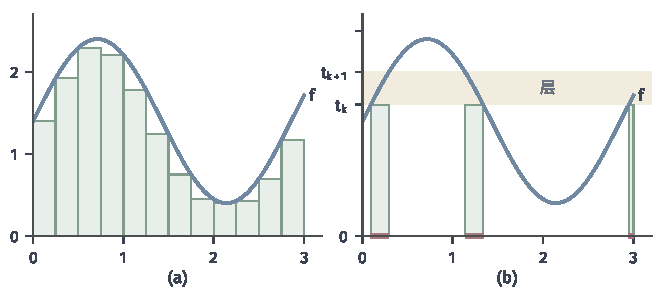
\includegraphics[width=112mm]{figures/04-spaces-measures-and-geometry/02-measure/matplotlib/integ-slicing-comparison/figure.pdf}
  \caption{同一函数$f(x)=1.4+\sin(2.2x)$的两种切法。(a)切定义域：把$[0,3]$等分成$12$段，绿色矩形以各段上$f$的下确界为高。(b)切值域：黄色带是值域区间$[1.6,2.0)$，红色线段是横轴上满足$1.6\leq f<2.0$的点，共三段，绿色矩形以$t_k=1.6$为高画在这些点上。}
  \label{fig:integ-slicing-comparison}
\end{BookInlineFigure}

下面先对只取有限个值的简单函数这样计算，再用简单函数从下方逼近一般的非负可测函数；随后用正负部分处理实值函数，用实部与虚部处理复值函数。

\subsection{非负积分}
\label{sec:integ-nonnegative}

\paragraph{简单函数的积分}
设$(X,\mathcal A,\mu)$是测度空间。非负简单函数在有限个不交可测集合上各取一个常值，分层已经现成，累计的方式就是“高度乘以测度”再求和。

由于测度可以为$+\infty$，先约定$0\cdot(+\infty)=0$：高度为零的层，无论占据多大的集合，贡献都是零。没有这条约定，$\mathbb R$上的零函数就没有积分。

\begin{definition}[非负简单函数的积分]
\label{def:integ-simple}
设$\varphi=\sum_{i=1}^mc_i\mathbf 1_{A_i}$是非负简单函数的标准表示，即$c_1,\dots,c_m\geq0$互不相同，$A_i=\{\varphi=c_i\}$。定义
\begin{equation}
 \int_X\varphi\,\mathrm d\mu=\sum_{i=1}^mc_i\,\mu(A_i)\in[0,+\infty].
 \label{eq:integ-simple}
\end{equation}
\end{definition}

图~\ref{fig:integ-simple-height}中$[0,3]$上的简单函数在$A_1=[0,1)\cup[2,2.5)$上取$2$，在$A_2=[1,2)\cup[2.5,3]$上取$0.5$。两层各占长度$1.5$，所以对Lebesgue测度的积分为
\[
 \int_{[0,3]}\varphi\,\mathrm d\lambda=2\times1.5+0.5\times1.5=3.75 .
\]
图下方的两行线段把两层在横轴上的位置单独画出。每一层都由不相邻的两段组成，而式~\eqref{eq:integ-simple}只用到它们的总长。

\begin{BookInlineFigure}
  \centering
  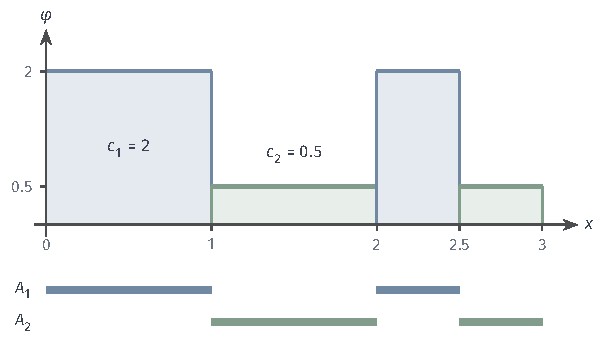
\includegraphics[width=102.401mm]{figures/04-spaces-measures-and-geometry/02-measure/tikz/integ-simple-height/figure.pdf}
  \caption{简单函数积分的“高度乘以测度”。$[0,3]$上的$\varphi$在$A_1=[0,1)\cup[2,2.5)$（蓝）上取$2$，在$A_2=[1,2)\cup[2.5,3]$（绿）上取$0.5$；下方两行线段标出两层占据的集合，各自总长为$1.5$。}
  \label{fig:integ-simple-height}
\end{BookInlineFigure}

同一个简单函数常常以别的方式写出，例如$[0,2]$的指示函数可以拆成$[0,1]$与$(1,2]$两段的指示函数之和。计算时我们希望随手把定义域切成方便的块，不必先合并成标准表示。下面的引理说明这样做得到同一个数，也给出简单函数积分的基本运算。

\begin{lemma}[简单函数积分的运算]
\label{lem:integ-simple-properties}
设$\varphi,\psi$是非负简单函数。
\begin{enumerate}
 \item 若$X$被分成两两不交的可测集$B_1,\dots,B_r$，$\varphi$在$B_j$上取常值$b_j$，则$\int\varphi\,\mathrm d\mu=\sum_jb_j\mu(B_j)$。
 \item 对$a,b\in[0,+\infty)$，有
 \begin{equation}
  \int(a\varphi+b\psi)\,\mathrm d\mu=a\int\varphi\,\mathrm d\mu+b\int\psi\,\mathrm d\mu .
  \label{eq:integ-simple-linear}
 \end{equation}
 \item 若$\varphi\leq\psi$，则$\varphi$的积分不超过$\psi$的积分。
 \item $E\mapsto\int\varphi\mathbf 1_E\,\mathrm d\mu$是$(X,\mathcal A)$上的测度。
\end{enumerate}
\end{lemma}

\begin{proof}
第1条。空的块对右端贡献为零，可以先去掉。设$\varphi$的标准表示为$\sum_ic_i\mathbf 1_{A_i}$，把取同一个值$c_i$的块合并，有
\[
 A_i=\bigcup_{j:\,b_j=c_i}B_j .
\]
由$\mu$的有限可加性，
\[
 \sum_jb_j\mu(B_j)=\sum_ic_i\sum_{j:\,b_j=c_i}\mu(B_j)=\sum_ic_i\mu(A_i).
\]

第2条。设$\varphi$的标准表示以$A_i$为块、取值$\alpha_i$，$\psi$的标准表示以$C_j$为块、取值$\beta_j$。集合$A_i\cap C_j$两两不交、并为$X$，$a\varphi+b\psi$在其上取常值$a\alpha_i+b\beta_j$。由第1条，
\[
 \int(a\varphi+b\psi)\,\mathrm d\mu=\sum_{i,j}(a\alpha_i+b\beta_j)\,\mu(A_i\cap C_j).
\]
把求和拆开，并对固定的$i$用有限可加性$\sum_j\mu(A_i\cap C_j)=\mu(A_i)$，对固定的$j$同样处理，得到
\[
 \int(a\varphi+b\psi)\,\mathrm d\mu=a\sum_i\alpha_i\mu(A_i)+b\sum_j\beta_j\mu(C_j).
\]

第3条。若$\varphi\leq\psi$，则在每个非空的$A_i\cap C_j$上$\alpha_i\leq\beta_j$。按这些块计算两个积分，再逐项比较即得。

第4条。函数$\varphi\mathbf 1_E$在$A_i\cap E$上取$c_i$，在$X\setminus E$上取$0$，由第1条，
\[
 \int\varphi\mathbf 1_E\,\mathrm d\mu=\sum_ic_i\,\mu(A_i\cap E).
\]
右端是有限个测度$E\mapsto\mu(A_i\cap E)$的非负加权和，由上一章的加权和规则，它是测度。
\end{proof}

\paragraph{一般非负函数的积分}
一般的非负可测函数可能取无穷多个值，没有有限分层可以直接计算。可行的办法是从下方逼近：若简单函数$\varphi$满足$0\leq\varphi\leq f$，它的积分就是$f$的累计的一个下界。上一章还证明了存在递增的简单函数列逐点趋于$f$，所以这些下界可以任意接近真正的累计。于是把全部下界的上确界定义为积分。

\begin{definition}[非负可测函数的积分]
\label{def:integ-nonnegative}
设$f:X\to[0,+\infty]$可测。定义
\begin{equation}
 \int_Xf\,\mathrm d\mu=\sup\Bigl\{\int_X\varphi\,\mathrm d\mu:\ \varphi\text{简单},\ 0\leq\varphi\leq f\Bigr\}.
 \label{eq:integ-nonnegative}
\end{equation}
值在$[0,+\infty]$中。常写作$\int f\,\mathrm d\mu$，或在不致混淆时写作$\int f$；对Lebesgue测度也写作$\int f(x)\,\mathrm dx$。
\end{definition}

这个定义与简单函数的积分不冲突。若$f$本身是简单函数，由引理~\ref{lem:integ-simple-properties}第3条，每个下方简单函数的积分都不超过$f$自己的积分，而$f$本身也是候选之一，所以上确界就是$f$自己的积分。

单调性可以直接从定义读出。若$0\leq f\leq g$，每个低于$f$的简单函数也低于$g$，上确界取在更大的范围上，于是$\int f\leq\int g$。

积分允许取$+\infty$。$\mathbb R$上$f\equiv1$的积分对Lebesgue测度为$\lambda(\mathbb R)=+\infty$。$(0,1]$上$f(x)=1/x$的积分也是$+\infty$：简单函数$\sum_{k=1}^nk\mathbf 1_{(1/(k+1),1/k]}$位于$f$下方，因为$(1/(k+1),1/k]$上$1/x\geq k$，而它的积分为
\[
 \sum_{k=1}^nk\Bigl(\frac1k-\frac1{k+1}\Bigr)=\sum_{k=1}^n\frac1{k+1},
\]
随$n$增大而无界。所以“积分有定义”与“积分有限”是两回事：非负函数的积分总有定义，但可能是$+\infty$。

\paragraph{递增逼近的积分}
定义用的是全部下方简单函数的上确界，这是一个庞大的集合。计算时我们只想用一列具体的逼近，例如上一章的二进分层逼近。下面的引理保证这样做不会漏掉任何下界。

\begin{lemma}[递增简单函数列的积分]
\label{lem:integ-increasing-simple}
设$f:X\to[0,+\infty]$可测，$\varphi_1\leq\varphi_2\leq\cdots$是非负简单函数，且对每个$x$有$\lim_n\varphi_n(x)=f(x)$。则
\begin{equation}
 \int_Xf\,\mathrm d\mu=\lim_{n\to\infty}\int_X\varphi_n\,\mathrm d\mu .
 \label{eq:integ-increasing-simple}
\end{equation}
\end{lemma}

\begin{proof}
积分$\int\varphi_n$关于$n$递增，并且都不超过$\int f$，所以极限存在且$\lim_n\int\varphi_n\leq\int f$。反方向要证明：对任意简单函数$0\leq s\leq f$，都有$\lim_n\int\varphi_n\geq\int s$。

固定$c\in(0,1)$，令$E_n=\{\varphi_n\geq cs\}$，它可测且关于$n$递增。下面说明$\bigcup_nE_n=X$。若$s(x)=0$，则$x\in E_1$。若$s(x)>0$，则$f(x)\geq s(x)>cs(x)$，而$\varphi_n(x)\to f(x)$，所以从某项起$\varphi_n(x)\geq cs(x)$。

由于$\varphi_n\geq cs\mathbf 1_{E_n}$，用单调性与线性性得到
\[
 \int\varphi_n\,\mathrm d\mu\geq c\int s\mathbf 1_{E_n}\,\mathrm d\mu .
\]
由引理~\ref{lem:integ-simple-properties}第4条，$E\mapsto\int s\mathbf 1_E\,\mathrm d\mu$是测度，集合$E_n$递增到$X$，所以由测度的从下连续性，右端趋于$c\int s\,\mathrm d\mu$。于是
\[
 \lim_n\int\varphi_n\,\mathrm d\mu\geq c\int s\,\mathrm d\mu .
\]
令$c\uparrow1$，得到所要的不等式。对$s$取上确界，即得$\lim_n\int\varphi_n\geq\int f$。
\end{proof}

引入因子$c<1$是为了处理$f(x)=s(x)$的点：在这些点上$\varphi_n(x)$可能永远略小于$s(x)$，却终究超过$cs(x)$。第~\ref{sec:integ-monotone-convergence}小节用一幅图看这件事，并把同一论证推广到一般的递增可测函数列。

\begin{example}[由定义计算$\int_{[0,1]}x\,\mathrm dx$]
\label{ex:integ-x-dyadic}
取$f(x)=x$，$x\in[0,1]$，测度为Lebesgue测度。二进分层逼近$\varphi_n$在$[k2^{-n},(k+1)2^{-n})$上取$k2^{-n}$，其中$0\leq k<2^n$；点$1$是零测集，在那里的取值不影响积分。每一层的宽度是$2^{-n}$，所以
\[
 \int\varphi_n\,\mathrm d\lambda=\sum_{k=0}^{2^n-1}\frac k{2^n}\cdot\frac1{2^n}=\frac1{4^n}\sum_{k=0}^{2^n-1}k .
\]
用等差数列求和$\sum_{k=0}^{2^n-1}k=\tfrac12(2^n-1)2^n$，得到
\[
 \int\varphi_n\,\mathrm d\lambda=\frac{(2^n-1)2^n}{2\cdot4^n}=\frac12\bigl(1-2^{-n}\bigr).
\]
前三项依次是
\[
 \frac14,\qquad\frac38,\qquad\frac7{16}.
\]
令$n\to\infty$，由引理~\ref{lem:integ-increasing-simple}得$\int_{[0,1]}x\,\mathrm dx=\frac12$，与黎曼积分的值相同。
\end{example}

图~\ref{fig:integ-dyadic-approx}画出了例子中的前三个逼近。绿色面积逐步填满直线下方的三角形。把第$n$步加细到第$n+1$步时，每个台阶右半边抬高$2^{-n-1}$，这些抬高部分的总面积是$2^{-n-2}$，正好是公式$\frac12(1-2^{-n})$的增量。

\begin{BookInlineFigure}
  \centering
  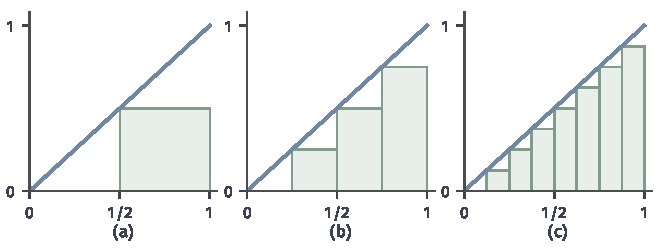
\includegraphics[width=112mm]{figures/04-spaces-measures-and-geometry/02-measure/matplotlib/integ-dyadic-approx/figure.pdf}
  \caption{$f(x)=x$（蓝）的二进分层逼近$\varphi_n$（绿色台阶）。(a)、(b)、(c)依次为$n=1,2,3$，绿色面积分别为$\frac14$、$\frac38$、$\frac7{16}$，递增趋于三角形面积$\frac12$。}
  \label{fig:integ-dyadic-approx}
\end{BookInlineFigure}

\paragraph{非负积分的可加性}
有了递增逼近，加法可以落到简单函数上完成。设$f,g$非负可测，取简单函数列$\varphi_n\uparrow f$与$\psi_n\uparrow g$，例如二进分层逼近。则$\varphi_n+\psi_n$是递增的非负简单函数，逐点收敛到$f+g$。由引理~\ref{lem:integ-increasing-simple}与引理~\ref{lem:integ-simple-properties}第2条，
\begin{equation}
\begin{aligned}
 \int(f+g)\,\mathrm d\mu&=\lim_n\int(\varphi_n+\psi_n)\,\mathrm d\mu\\
 &=\lim_n\int\varphi_n\,\mathrm d\mu+\lim_n\int\psi_n\,\mathrm d\mu\\
 &=\int f\,\mathrm d\mu+\int g\,\mathrm d\mu .
\end{aligned}
 \label{eq:integ-nonnegative-additive}
\end{equation}
用$c\varphi_n\uparrow cf$同样得到$\int cf=c\int f$，其中$c\in[0,+\infty)$。这些等式在$[0,+\infty]$中成立，允许两边为$+\infty$；系数取$+\infty$的情形放在第~\ref{sec:integ-linearity}小节核对。

\subsection{有符号积分}
\label{sec:integ-signed}

\paragraph{正部与负部}
取正负值的函数，正的贡献与负的贡献会相互抵消。若把两者混在一起累计，结果可能取决于累计的先后。最稳妥的做法是把两种贡献分开累计，最后再相减。对可测函数$f:X\to[-\infty,+\infty]$，令
\begin{equation}
 f^+=\max\{f,0\},\qquad f^-=\max\{-f,0\}.
 \label{eq:integ-parts}
\end{equation}
它们是非负可测函数，每一点至少一个为零，并且满足
\[
 f=f^+-f^-,\qquad \lvert f\rvert=f^++f^- .
\]
图~\ref{fig:integ-positive-negative-parts}以$\sin x$为例：$f^+$保留上半部分，$f^-$把下半部分翻到横轴上方。

\begin{BookInlineFigure}
  \centering
  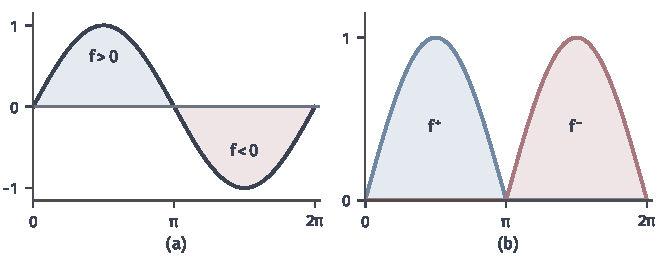
\includegraphics[width=112mm]{figures/04-spaces-measures-and-geometry/02-measure/matplotlib/integ-positive-negative-parts/figure.pdf}
  \caption{正负部分解，$f(x)=\sin x$，$x\in[0,2\pi]$。(a)$f$在$[0,\pi]$上为正（蓝底），在$[\pi,2\pi]$上为负（红底）。(b)正部$f^+$（蓝）与负部$f^-$（红）都是非负函数，每一点至少一个为零。}
  \label{fig:integ-positive-negative-parts}
\end{BookInlineFigure}

分开累计之后，两部分的积分都有意义，唯一的障碍是相减时可能出现$+\infty-(+\infty)$。下面的定义把这种情形排除在外。

\begin{definition}[积分存在与可积]
\label{def:integ-signed}
设$f:X\to[-\infty,+\infty]$可测。若$\int f^+\,\mathrm d\mu$与$\int f^-\,\mathrm d\mu$中至少一个有限，称$f$的积分存在，定义
\begin{equation}
 \int_Xf\,\mathrm d\mu=\int_Xf^+\,\mathrm d\mu-\int_Xf^-\,\mathrm d\mu\in[-\infty,+\infty].
 \label{eq:integ-signed}
\end{equation}
若$\int\lvert f\rvert\,\mathrm d\mu<+\infty$，称$f$关于$\mu$\term{可积}（integrable），也称\term{Lebesgue可积}（Lebesgue integrable），此时积分称为$f$的\term{Lebesgue积分}（Lebesgue integral）。
\end{definition}

三种情形可以这样区分。在$\mathbb R$上取$f=\mathbf 1_{[0,+\infty)}-\mathbf 1_{(-\infty,0)}$，正部与负部的积分都是$+\infty$，$f$的积分不存在；不能因为图像左右对称就说积分为零，那需要额外指定一种抵消的次序。取$f=\mathbf 1_{[0,+\infty)}$，积分存在且等于$+\infty$，但$f$不可积。取$f=\mathbf 1_{[0,1]}-\mathbf 1_{[-2,-1]}$，两部分的积分都是$1$，$f$可积且积分为$0$。

可积性用$\lvert f\rvert$规定，由$\lvert f\rvert=f^++f^-$与式~\eqref{eq:integ-nonnegative-additive}得
\[
 \int\lvert f\rvert\,\mathrm d\mu=\int f^+\,\mathrm d\mu+\int f^-\,\mathrm d\mu .
\]
所以$\int\lvert f\rvert<+\infty$当且仅当两部分的积分都有限。此时$\int f$是有限实数，并且
\[
 \Bigl\lvert\int f\,\mathrm d\mu\Bigr\rvert\leq\int f^+\,\mathrm d\mu+\int f^-\,\mathrm d\mu=\int\lvert f\rvert\,\mathrm d\mu .
\]

\paragraph{零测集与几乎处处等价类}
非负积分对零测集“视而不见”，这是用测度累计的直接后果：零测集这一层，高度再大，贡献也是零。下面的引理把这一点说清楚，并说明积分只依赖函数的几乎处处等价类。

\begin{lemma}[非负积分与零测集]
\label{lem:integ-null-sets}
设$f,g:X\to[0,+\infty]$可测。
\begin{enumerate}
 \item 对$t>0$，$\mu(\{f\geq t\})\leq\frac1t\int f\,\mathrm d\mu$。
 \item 若$\int f\,\mathrm d\mu<+\infty$，则$f<+\infty$几乎处处成立。
 \item $\int f\,\mathrm d\mu=0$当且仅当$f=0$几乎处处成立。
 \item 若$f=g$几乎处处成立，则$\int f\,\mathrm d\mu=\int g\,\mathrm d\mu$。
\end{enumerate}
\end{lemma}

\begin{proof}
第1条。$t\mathbf 1_{\{f\geq t\}}$是低于$f$的简单函数，它的积分是$t\mu(\{f\geq t\})$，所以$t\mu(\{f\geq t\})\leq\int f$。

第2条。对一切$t>0$有$\{f=+\infty\}\subseteq\{f\geq t\}$，由第1条，
\[
 \mu(\{f=+\infty\})\leq\frac1t\int f\,\mathrm d\mu .
\]
令$t\to+\infty$，右端趋于$0$。

第3条。若$\int f=0$，由第1条，对每个正整数$k$有$\mu(\{f\geq1/k\})=0$。又$\{f>0\}=\bigcup_k\{f\geq1/k\}$，所以$\mu(\{f>0\})=0$。反过来，设$N=\{f>0\}$零测。任一低于$f$的简单函数在$N$外为零，它的非零各层都含于$N$，测度为零，所以积分为$0$，上确界也是$0$。

第4条。设$N$是零测集，$f,g$在$N$外相等。对低于$f$的简单函数$\varphi$，函数$\varphi\mathbf 1_{X\setminus N}$低于$g$。由引理~\ref{lem:integ-simple-properties}第4条，
\[
 \int\varphi\,\mathrm d\mu=\int\varphi\mathbf 1_{X\setminus N}\,\mathrm d\mu+\int\varphi\mathbf 1_N\,\mathrm d\mu .
\]
最后一项按层计算为零，所以$\int\varphi\leq\int g$。对$\varphi$取上确界得$\int f\leq\int g$，对称地得到反向不等式。
\end{proof}

第1条称为\term{Markov不等式}（Markov inequality），它用积分控制函数取大值的集合有多大。在$[0,1]$上取$f(x)=x$、$t=\frac12$，左边是$\lambda(\{x\geq\frac12\})=\frac12$，右边是$2\cdot\frac12=1$，不等式成立。

对实值函数，若$f=g$几乎处处成立，则$f^\pm=g^\pm$几乎处处成立，由第4条，两者的积分存在性、可积性和积分值都相同。所以积分是定义在几乎处处等价类上的：在零测集上改动函数，或者在零测集上根本不给函数赋值，都不影响积分。

可积函数的取值可以是$\pm\infty$，但由第2条只能发生在零测集上，因此总可以改成处处取实数值的可积函数而积分不变。把可积函数按几乎处处相等分类，得到的空间及其范数结构在第~\ref{chap:function-normed-spaces}章研究。

\subsection{复值积分}
\label{sec:integ-complex}

\paragraph{复值可测函数的可积性}
Fourier分析中的$e^{\mathrm ikx}$、内积$\int\bar fg$都是复值的，所以积分要推广到复值函数。设$f=u+\mathrm iv:X\to\mathbb C$，其中$u,v$为实值可测函数，上一章已说明$\lvert f\rvert=\sqrt{u^2+v^2}$可测。复数没有正负之分，不能再用正部负部拆开；可以把它看成平面上的向量，分别累计两个坐标，而可积性仍用非负函数$\lvert f\rvert$规定。

\begin{definition}[复值函数的积分]
\label{def:integ-complex}
设$f=u+\mathrm iv$是复值可测函数。若$\int\lvert f\rvert\,\mathrm d\mu<+\infty$，称$f$可积，并定义
\begin{equation}
 \int_Xf\,\mathrm d\mu=\int_Xu\,\mathrm d\mu+\mathrm i\int_Xv\,\mathrm d\mu .
 \label{eq:integ-complex}
\end{equation}
\end{definition}

定义右端要求$u,v$都可积，下面的引理说明这正好由$\lvert f\rvert$可积保证。

\begin{lemma}[复值可积性的等价刻画]
\label{lem:integ-complex-integrable}
复值可测函数$f=u+\mathrm iv$可积，当且仅当$u$与$v$都可积。
\end{lemma}

\begin{proof}
平面上一个向量的长度不小于每个坐标的绝对值，不大于两个坐标绝对值之和，所以逐点有
\[
 \lvert u\rvert\leq\lvert f\rvert,\qquad\lvert v\rvert\leq\lvert f\rvert,\qquad\lvert f\rvert\leq\lvert u\rvert+\lvert v\rvert .
\]
若$\int\lvert f\rvert<+\infty$，由非负积分的单调性，$\int\lvert u\rvert$与$\int\lvert v\rvert$都有限。反过来，由单调性与式~\eqref{eq:integ-nonnegative-additive}，
\[
 \int\lvert f\rvert\,\mathrm d\mu\leq\int\lvert u\rvert\,\mathrm d\mu+\int\lvert v\rvert\,\mathrm d\mu<+\infty.
\]
\end{proof}

\paragraph{共轭与几乎处处相等}
复共轭$\bar f=u-\mathrm iv$与$f$的模相同，所以$\bar f$可积当且仅当$f$可积。由定义~\ref{def:integ-complex}直接得到
\[
 \int\bar f\,\mathrm d\mu=\int u\,\mathrm d\mu-\mathrm i\int v\,\mathrm d\mu=\overline{\int f\,\mathrm d\mu}.
\]
若复值函数$f,g$几乎处处相等，则实部、虚部分别几乎处处相等，由第~\ref{sec:integ-signed}小节，两者的积分相同。所以复值积分同样只依赖几乎处处等价类。

\begin{example}[复值积分的抵消]
\label{ex:integ-complex-cancel}
取$X=\{1,2,3,4\}$，每点质量$1/4$，$f(k)=\mathrm i^k$。实部$u$依次为$0,-1,0,1$，虚部$v$依次为$1,0,-1,0$。分别累计两个坐标：
\[
 \int u\,\mathrm d\mu=\frac14(0-1+0+1)=0,\qquad\int v\,\mathrm d\mu=\frac14(1+0-1+0)=0 .
\]
于是$\int f\,\mathrm d\mu=0$。另一方面$\lvert f\rvert\equiv1$，$\int\lvert f\rvert\,\mathrm d\mu=1$。四个方向的单位复数相互抵消，积分的模远小于模的积分。
\end{example}

复值积分把实值情形的运算搬到两个坐标上，不再比较大小。第~\ref{chap:function-inner-product-spaces}章的$L^2$内积$\langle f,g\rangle=\int f\bar g\,\mathrm d\mu$、第~\ref{chap:fourier-transform}章的Fourier系数与Fourier变换，都以这里的复值积分及其共轭规则为共同运算。

\section{积分的基本性质}
\label{sec:integ-basic-properties}

计算积分时我们反复做三件事：把被积函数拆成几项分别积分，用一个容易计算的函数从上方或下方比较，把积分区域切成几块分别累计。在有限情形$\sum_if(i)\mu_i$里，这三件事分别对应求和的线性、逐项比较和分组求和，都没有条件。

积分的情形多了一个麻烦：值可以是$+\infty$，而$+\infty-(+\infty)$没有意义。所以下面每条规则都要写明范围：可积函数的运算在有限实数中进行，非负函数允许积分为$+\infty$，但不允许系数为负。

\subsection{线性性}
\label{sec:integ-linearity}

\paragraph{三种情形的线性性}
线性性要回答两件事：线性组合是否仍属于可以积分的范围，积分能否逐项计算。非负函数总可以积分，但系数必须非负，否则会产生负值；可积函数允许任意实系数或复系数，代价是要先核对线性组合仍然可积。

\begin{theorem}[积分的线性性]
\label{thm:integ-linearity}
\begin{enumerate}
 \item 设$f,g:X\to[0,+\infty]$可测，$a,b\in[0,+\infty]$，约定$0\cdot(+\infty)=0$。则下式在$[0,+\infty]$中成立：
 \begin{equation}
  \int(af+bg)\,\mathrm d\mu=a\int f\,\mathrm d\mu+b\int g\,\mathrm d\mu .
  \label{eq:integ-linearity}
 \end{equation}
 \item 设$f,g$是实值可积函数，$a,b\in\mathbb R$。则$af+bg$可积，且式~\eqref{eq:integ-linearity}成立。
 \item 设$f,g$是复值可积函数，$a,b\in\mathbb C$。则$af+bg$可积，且式~\eqref{eq:integ-linearity}成立。
\end{enumerate}
\end{theorem}

\begin{proof}
第1条。由式~\eqref{eq:integ-nonnegative-additive}，$\int(af+bg)=\int af+\int bg$，所以只需证明$\int af=a\int f$。系数有限的情形第~\ref{sec:integ-nonnegative}小节已经给出，只需处理$a=+\infty$。

函数$(+\infty)\cdot f$在$\{f>0\}$上取$+\infty$，在$\{f=0\}$上取$0$。分两种情形。若$\mu(\{f>0\})>0$，这个函数的积分为$+\infty$；由引理~\ref{lem:integ-null-sets}第3条，此时$\int f>0$，右端$(+\infty)\cdot\int f$也是$+\infty$。若$\mu(\{f>0\})=0$，左端是几乎处处为零的函数的积分，等于$0$；右端是$(+\infty)\cdot0=0$。

第2条，先看可积性。可积函数只在零测集上取$\pm\infty$，把这些点上的值改成$0$，积分不变，$af+bg$处处有定义。由三角不等式与第1条，
\[
 \int\lvert af+bg\rvert\,\mathrm d\mu\leq\lvert a\rvert\int\lvert f\rvert\,\mathrm d\mu+\lvert b\rvert\int\lvert g\rvert\,\mathrm d\mu<+\infty,
\]
所以$af+bg$可积。

再看数乘。$a\geq0$时$(af)^\pm=af^\pm$；$a<0$时$(af)^+=\lvert a\rvert f^-$，$(af)^-=\lvert a\rvert f^+$。代入式~\eqref{eq:integ-signed}，两种情形都得到$\int af=a\int f$。

最后看加法。令$h=f+g$。把$h^+-h^-=f^+-f^-+g^+-g^-$中带负号的项移到另一边，得到
\[
 h^++f^-+g^-=h^-+f^++g^+ .
\]
两边都是非负可测函数之和，由第1条逐项积分，六个积分都有限，于是可以移项，得到
\[
 \int h\,\mathrm d\mu=\int f\,\mathrm d\mu+\int g\,\mathrm d\mu .
\]

第3条。第2条中的三角不等式对复数同样成立，给出可积性。加法按实部与虚部分别用第2条。对复数$a=\alpha+\mathrm i\beta$与$f=u+\mathrm iv$，有
\[
 af=(\alpha u-\beta v)+\mathrm i(\alpha v+\beta u).
\]
由第2条分别积分实部与虚部，再合并成复数的乘积：
\[
\begin{aligned}
 \int af&=\alpha\int u-\beta\int v+\mathrm i\Bigl(\alpha\int v+\beta\int u\Bigr)\\
 &=(\alpha+\mathrm i\beta)\Bigl(\int u+\mathrm i\int v\Bigr)=a\int f.
\end{aligned}
\]
\end{proof}

\paragraph{条件不能省略}
第2条要求两个函数都可积，只知道各自的积分存在是不够的。在$\mathbb R$上取$f\equiv1$、$g\equiv-1$，两者的积分分别为$+\infty$与$-\infty$，都存在。而$f+g\equiv0$的积分为$0$，右端却是$+\infty+(-\infty)$，没有意义。

第1条要求系数非负，同样是为了不让正负贡献相遇。由第2条，可积函数全体对线性组合封闭，积分是其上的线性映射，就像有限维时$f\mapsto\sum_if(i)\mu_i$是一个线性函数。这一结构在第~\ref{chap:function-normed-spaces}章作为函数空间再研究。

\subsection{单调性}
\label{sec:integ-monotonicity}

\paragraph{逐点比较}
用一个已知的函数控制被积函数，是估计积分最常用的办法。非负函数的单调性已由定义得到；对实值可积函数，比较可以借助线性性完成：$f\leq g$意味着$g-f\geq0$，非负函数的积分非负。

\begin{theorem}[积分的单调性]
\label{thm:integ-monotonicity}
设$f,g$都是非负可测函数，或都是实值可积函数。若$f\leq g$几乎处处成立，则$\int f\,\mathrm d\mu\leq\int g\,\mathrm d\mu$。若还有$\int f=\int g$且两者有限，则$f=g$几乎处处成立。
\end{theorem}

\begin{proof}
设$N$是零测集，$f\leq g$在$N$外成立。把$f,g$在$N$上都改成$0$，由引理~\ref{lem:integ-null-sets}第4条（实值情形对正负部分别使用），积分不变，而改后的函数处处满足$f\leq g$。

非负情形由定义的单调性得结论。可积情形中，$g-f$是几乎处处非负的可积函数，由线性性，
\[
 \int g\,\mathrm d\mu-\int f\,\mathrm d\mu=\int(g-f)\,\mathrm d\mu\geq0 .
\]

现在设两个积分相等且有限。非负情形下$f,g$的积分有限，也属于可积函数，所以统一按可积情形处理。这时$\int(g-f)=0$，而$g-f$几乎处处非负，由引理~\ref{lem:integ-null-sets}第3条，$g-f=0$几乎处处成立。
\end{proof}

逐点不等式放宽到几乎处处，是因为积分看不见零测集上的取值。例如在$[0,1]$上，$\mathbf 1_{\mathbb Q}\leq0$只在零测的有理点之外成立，结论$\int\mathbf 1_{\mathbb Q}\leq0$仍然正确，再结合$\mathbf 1_{\mathbb Q}\geq0$，得$\int\mathbf 1_{\mathbb Q}=0$。

\paragraph{复值积分不比较大小}
复数之间没有与运算相容的次序，所以复值积分没有单调性可言。能比较的是实值量：实部与虚部满足$\operatorname{Re}\int f=\int\operatorname{Re}f$，可以对它们分别使用单调性；模$\lvert f\rvert$是非负函数，也可以比较。下一小节就是用实部与模的比较来估计复值积分。

\subsection{积分的绝对值估计}
\label{sec:integ-absolute-estimate}

\paragraph{实值与复值情形}
积分是加权累计，取绝对值之后，正负或不同方向的贡献不再抵消，累计只会变大。这与向量的三角不等式$\lVert\sum_iv_i\rVert\leq\sum_i\lVert v_i\rVert$是同一件事：把许多向量首尾相接，总位移不超过路程之和。

\begin{theorem}[积分的绝对值估计]
\label{thm:integ-absolute-estimate}
设$f$是实值或复值可积函数，则
\begin{equation}
 \Bigl\lvert\int f\,\mathrm d\mu\Bigr\rvert\leq\int\lvert f\rvert\,\mathrm d\mu .
 \label{eq:integ-absolute-estimate}
\end{equation}
\end{theorem}

\begin{proof}
实值情形。由$-\lvert f\rvert\leq f\leq\lvert f\rvert$与单调性、线性性，
\[
 -\int\lvert f\rvert\,\mathrm d\mu\leq\int f\,\mathrm d\mu\leq\int\lvert f\rvert\,\mathrm d\mu .
\]

复值情形。记$z=\int f\,\mathrm d\mu$。若$z=0$，左端为零，不等式成立。若$z\neq0$，令$\alpha=\bar z/\lvert z\rvert$，这是模为一的复数，使$\alpha z=\lvert z\rvert$为正实数。由复线性性，
\[
 \lvert z\rvert=\alpha\int f\,\mathrm d\mu=\int\alpha f\,\mathrm d\mu .
\]
左边是实数，所以它等于右边的实部。再用复数的实部不超过它的模这一事实与单调性，并利用$\lvert\alpha\rvert=1$，得到
\[
 \lvert z\rvert=\int\operatorname{Re}(\alpha f)\,\mathrm d\mu\leq\int\lvert\alpha f\rvert\,\mathrm d\mu=\int\lvert f\rvert\,\mathrm d\mu .
\]
\end{proof}

证明中乘以$\alpha$的作用是把积分旋转到正实轴上，这样复数的模就变成了可以比较大小的实部。例~\ref{ex:integ-complex-cancel}中$\lvert\int f\rvert=0<1=\int\lvert f\rvert$，说明不等式可以严格成立：四个向量首尾相接回到原点，总位移为零，路程却是$1$。

\paragraph{误差控制}
把估计用于两个可积函数之差，就得到积分误差的界：
\begin{equation}
 \Bigl\lvert\int f\,\mathrm d\mu-\int g\,\mathrm d\mu\Bigr\rvert\leq\int\lvert f-g\rvert\,\mathrm d\mu .
 \label{eq:integ-error-bound}
\end{equation}
用$g$近似$f$时，积分结果的误差不超过两者差的模的积分。

用例~\ref{ex:integ-x-dyadic}的二进分层函数检验这个界。在$[0,1]$上用$\varphi_n$近似$f(x)=x$，逐点有$0\leq f-\varphi_n\leq2^{-n}$，所以式~\eqref{eq:integ-error-bound}的右端不超过$2^{-n}$。实际误差是
\[
 \frac12-\frac12\bigl(1-2^{-n}\bigr)=2^{-n-1},
\]
确实在这个界之内。第~\ref{sec:integ-dominated-convergence}小节将用同一个量$\int\lvert f_n-f\rvert$判断一列近似的积分是否收敛。

\subsection{积分区域的可加性}
\label{sec:integ-domain-additivity}

\paragraph{子集上的积分}
在可测子集$A$上积分，就是只累计$A$内的贡献。用指示函数把$A$外的值清零，就可以沿用全空间上的定义。

\begin{definition}[可测子集上的积分]
\label{def:integ-subset}
设$A\in\mathcal A$，$f$非负可测或可积。定义
\begin{equation}
 \int_Af\,\mathrm d\mu=\int_Xf\mathbf 1_A\,\mathrm d\mu .
 \label{eq:integ-subset}
\end{equation}
对Lebesgue测度和区间$A=[a,b]$，也写作$\int_a^bf(x)\,\mathrm dx$。
\end{definition}

这个积分也等于把$f$限制到$A$上、在$A$的可测子集族上对$\mu$所作的积分，因为两种算法在简单函数上逐层相同，再由递增逼近推广到一般函数。若$f$可积，由$\lvert f\mathbf 1_A\rvert\leq\lvert f\rvert$，$f$在每个可测子集上可积。

\paragraph{有限拆分与零测集}
设$A,B\in\mathcal A$不交。则$f\mathbf 1_{A\cup B}=f\mathbf 1_A+f\mathbf 1_B$，由线性性，
\begin{equation}
 \int_{A\cup B}f\,\mathrm d\mu=\int_Af\,\mathrm d\mu+\int_Bf\,\mathrm d\mu .
 \label{eq:integ-domain-additive}
\end{equation}
这对非负可测函数在$[0,+\infty]$中成立，对可积函数在有限数中成立；归纳可得有限个不交区域的情形。

若$N$是零测集，$f\mathbf 1_{A\cup N}$与$f\mathbf 1_A$只在$N$上可能不同，所以$\int_{A\cup N}f=\int_Af$。增删零测集不改变积分，区间端点开闭也就无关紧要：$\int_{[a,b]}f=\int_{(a,b)}f$。

\paragraph{可数拆分}
可数个不交区域$A_1,A_2,\dots$的情形不能从有限拆分直接得到，因为需要交换积分与无限求和。对非负可测函数，第~\ref{sec:integ-monotone-convergence}小节的单调收敛定理将给出
\begin{equation}
 \int_{\bigcup_nA_n}f\,\mathrm d\mu=\sum_n\int_{A_n}f\,\mathrm d\mu,
 \label{eq:integ-domain-countable}
\end{equation}
两边允许为$+\infty$；对可积函数，再由支配收敛得到同样的等式且级数绝对收敛。换句话说，对非负可测函数$f$，$A\mapsto\int_Af\,\mathrm d\mu$本身是一个测度。由非负函数生成的这类测度怎样反过来刻画，放在第~\ref{chap:measure-densities}章。

\section{与经典积分的关系}
\label{sec:integ-classical}

新积分的定义与黎曼积分完全不同：一个切值域，一个切定义域。对熟悉的区间积分，两种定义给出的数是否相同，新积分又多处理了哪些函数？

本节分两种情形比较。有界闭区间上的有界函数，用不连续点集刻画黎曼可积性并证明两种积分相等；无界区间或奇点附近的反常积分，绝对收敛时与新积分一致，条件收敛时则不然。下文中区间上的测度都是Lebesgue测度$\lambda$。

\subsection{与黎曼积分的关系}
\label{sec:integ-riemann}

\paragraph{阶梯函数与上下和}
两种理论的接触点是阶梯函数。对区间$I\subseteq[a,b]$，$\int\mathbf 1_I\,\mathrm d\lambda=\lambda(I)$等于区间长度，与黎曼积分的值相同；端点是零测集，开闭不影响Lebesgue积分。由线性性，阶梯函数$\sum_ic_i\mathbf 1_{I_i}$的两种积分都等于$\sum_ic_i\lambda(I_i)$。而黎曼积分的上和与下和正是阶梯函数的积分，两种理论就从这里连起来。

回顾卷一的Darboux判据：有界函数$f$在$[a,b]$上黎曼可积，当且仅当对任意$\varepsilon>0$存在分割$P$，使上和与下和之差$U(f,P)-L(f,P)<\varepsilon$；此时黎曼积分是上下和共同逼近的值（可参考\BookChapterRef{chap:univariate-integration}{卷一第7章“一元函数的积分”}）。下面的判据把“上下和之差可以任意小”换成一个关于不连续点的测度条件。

\paragraph{振幅与不连续点}
上下和之差由函数在小段上的跳动幅度决定，所以要先量化函数在一点附近的跳动。设$f:[a,b]\to\mathbb R$有界，记$I_\delta(x)=(x-\delta,x+\delta)\cap[a,b]$，定义$f$在$x$处的\term{振幅}（oscillation）
\begin{equation}
 \omega_f(x)=\inf_{\delta>0}\Bigl(\sup_{I_\delta(x)}f-\inf_{I_\delta(x)}f\Bigr).
 \label{eq:integ-oscillation}
\end{equation}
括号内的量随$\delta$减小而不增，下确界就是$\delta\downarrow0$时的极限。$f$在$x$连续当且仅当$\omega_f(x)=0$，所以不连续点集为$D_f=\bigcup_{m\geq1}\{\omega_f\geq1/m\}$。例如$\mathbf 1_{[1/2,1]}$在$x=\frac12$处的振幅是$1$，在其余点都是$0$。

有了振幅，可以陈述下面的判据：决定黎曼可积性的是不连续点集的测度。

\begin{theorem}[黎曼可积的Lebesgue判据]
\label{thm:integ-riemann-lebesgue}
设$f:[a,b]\to\mathbb R$有界。$f$黎曼可积，当且仅当其不连续点集$D_f$是Lebesgue零测集。此时$f$关于Lebesgue可测集可测，Lebesgue可积，且$\int_{[a,b]}f\,\mathrm d\lambda$等于$f$的黎曼积分。
\end{theorem}

这一判据称为\term{Lebesgue判据}（Lebesgue criterion）。证明分三步：先说明黎曼可积函数被两列阶梯函数夹住，由此得到两种积分相等；再读出$D_f$零测；最后由$D_f$零测构造上下和之差很小的分割。下面始终记$\lvert f\rvert\leq M$。

\begin{proof}
\emph{第一步：两种积分相等。}设$f$黎曼可积。由Darboux判据，对每个$k$有分割$Q_k$使上下和之差小于$1/k$。令$P_k$为$Q_1,\dots,Q_k$的公共加细，加细不增大上下和之差，于是$P_1\subseteq P_2\subseteq\cdots$，且$U(f,P_k)-L(f,P_k)\to0$。

对$P_k$的每个小段$[x_{i-1},x_i]$，记$m_i,M_i$为$f$在其上的下、上确界，令$J_i=[x_{i-1},x_i)$（最后一段取闭区间），定义阶梯函数
\[
 \varphi_k=\sum_im_i\mathbf 1_{J_i},\qquad\psi_k=\sum_iM_i\mathbf 1_{J_i}.
\]
于是$\varphi_k\leq f\leq\psi_k$，并且
\[
 \int\varphi_k\,\mathrm d\lambda=L(f,P_k),\qquad\int\psi_k\,\mathrm d\lambda=U(f,P_k).
\]

分割加细时子段上的下确界不减、上确界不增，所以$\varphi_k$递增、$\psi_k$递减，分别有逐点极限$\varphi\leq f\leq\psi$，它们都是Borel可测函数。由$0\leq\psi-\varphi\leq\psi_k-\varphi_k$，得到
\[
 \int(\psi-\varphi)\,\mathrm d\lambda\leq U(f,P_k)-L(f,P_k)\to0 .
\]
所以$\psi=\varphi$在某个零测集$N$外成立，从而$f=\varphi$在$N$外成立。

集合$\{f>t\}$与Borel集$\{\varphi>t\}$只在$N$内可能不同，Lebesgue测度完备，所以$f$关于$\mathcal L$可测；又$\lvert f\rvert\leq M$，$f$在有限长区间上可积。$\varphi_k+M$是递增的非负简单函数，逐点收敛到$\varphi+M$，由引理~\ref{lem:integ-increasing-simple}，$\int(\varphi_k+M)\to\int(\varphi+M)$。两边减去有限数$M(b-a)$，得到
\[
 \int_{[a,b]}f\,\mathrm d\lambda=\int_{[a,b]}\varphi\,\mathrm d\lambda=\lim_kL(f,P_k)=\int_a^bf(x)\,\mathrm dx .
\]

\emph{第二步：$D_f$零测。}全部分割$P_k$的分点只有可数个，组成零测集$Z$。若$x\notin Z$，对每个$k$，$x$位于$P_k$某个小段的内部，存在$\delta$使$I_\delta(x)$含于该小段，于是
\[
 \omega_f(x)\leq M_i-m_i=\psi_k(x)-\varphi_k(x).
\]
令$k\to\infty$得$\omega_f(x)\leq\psi(x)-\varphi(x)$。在零测集$Z\cup N$之外右端为零，所以$D_f\subseteq Z\cup N$是零测集。

\emph{第三步：$D_f$零测蕴含黎曼可积。}给定$\varepsilon>0$，令$K=\{\omega_f\geq\varepsilon\}$。$K$是闭集：若$\omega_f(x)<\varepsilon$，取$\delta$使$I_\delta(x)$上上下确界之差小于$\varepsilon$，则对$\lvert y-x\rvert<\delta/2$有$I_{\delta/2}(y)\subseteq I_\delta(x)$，故$\omega_f(y)<\varepsilon$。

$K\subseteq D_f$是零测的有界闭集，可用可数个开区间覆盖且总长小于$\varepsilon$。$K$紧，取其中有限个，其并$G$由有限个不交开区间组成，总长小于$\varepsilon$。于是$[a,b]\setminus G$是有限个闭区间$H_1,\dots,H_r$之并，其上处处$\omega_f<\varepsilon$。

对每点$x\in H_l$取$\delta_x$，使$I_{\delta_x}(x)$上上下确界之差小于$\varepsilon$。区间$(x-\delta_x/2,x+\delta_x/2)$覆盖紧集$H_l$，取有限子覆盖，令$\delta$为相应$\delta_x/2$的最小值。若$H_l$中的小段$J$长度小于$\delta$，它含于某个$I_{\delta_x}(x)$，$f$在$J$上的上下确界之差小于$\varepsilon$。

把每个$H_l$分成长度小于$\delta$的小段，再加上$G$各分支的端点，得到分割$P$。上下和之差分两部分估计：落在某个$H_l$中的小段，每段的上下确界之差小于$\varepsilon$，总长不超过$b-a$，贡献小于$\varepsilon(b-a)$；落在$G$某个分支闭包中的小段，上下确界之差至多$2M$，总长小于$\varepsilon$，贡献至多$2M\varepsilon$。于是
\[
 U(f,P)-L(f,P)<\varepsilon(b-a+2M),
\]
由Darboux判据，$f$黎曼可积。
\end{proof}

第一步说明两种理论在共同范围内一致：黎曼可积函数的上下阶梯函数从两侧夹住它，Lebesgue积分记录了夹逼的公共极限。第二、三步说明黎曼可积的障碍恰好是不连续点占据正的长度。

这里用到了完备性。黎曼可积函数未必Borel可测，但与一个Borel函数只在零测集上不同，所以结论说的是关于Lebesgue可测集$\mathcal L$可测。

\paragraph{有理点指示函数}
在$[0,1]$上，有理点的指示函数$\mathbf 1_{\mathbb Q}$称为\term{Dirichlet函数}（Dirichlet function）。$\mathbb Q\cap[0,1]$可数，Lebesgue测度为零，所以
\[
 \int_{[0,1]}\mathbf 1_{\mathbb Q}\,\mathrm d\lambda=0 .
\]
另一方面，每个小区间上它的上确界为$1$、下确界为$0$，振幅处处为$1$，$D_f=[0,1]$的测度为$1$，所以它不黎曼可积。这与“任意分割的下和为$0$、上和为$1$”的直接计算一致。

图~\ref{fig:integ-dirichlet-function}把这个例子与Cantor集的指示函数放在一起。Cantor集$C$是零测的闭集，$\mathbf 1_C$在每个$x\notin C$的邻域内恒为零，因而连续；在$x\in C$处，由于$C$不含任何区间，$x$附近有取值为零的点，因而不连续。于是$D_f=C$不可数却零测，$\mathbf 1_C$黎曼可积，两种积分都是$0$。

\begin{BookInlineFigure}
  \centering
  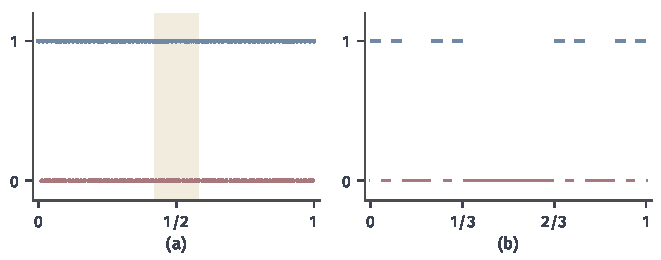
\includegraphics[width=112mm]{figures/04-spaces-measures-and-geometry/02-measure/matplotlib/integ-dirichlet-function/figure.pdf}
  \caption{两种不连续点集。(a)Dirichlet函数在有理点取$1$（蓝点）、无理点取$0$（红点），图中各取若干代表；两类点都稠密，任一小区间（黄色带）上上确界为$1$、下确界为$0$，不连续点集为整个$[0,1]$。(b)Cantor集的指示函数$\mathbf 1_C$，用第三步的$8$个保留区间示意$C$：蓝色线段处取$1$，红色线段处取$0$。它只在$C$上不连续，$\lambda(C)=0$，所以黎曼可积。}
  \label{fig:integ-dirichlet-function}
\end{BookInlineFigure}

两张图的对比说明，决定黎曼可积性的是不连续点集的测度，而不是它的基数或稠密性。$\mathbb Q$的基数比$C$小，$\mathbf 1_{\mathbb Q}$却不黎曼可积，因为它的不连续点集是全区间。Lebesgue积分则根本不要求函数在小区间上近似为常数，只要求各层可测。

\subsection{与反常积分的关系}
\label{sec:integ-improper}

\paragraph{截断区间的极限}
反常积分处理两种情形：区间无界，或函数在端点附近无界。做法都是先在有限闭区间上作黎曼积分，再让区间扩张取极限。新积分则直接在整个区间上累计，不需要截断。对非负函数，截断区间上的积分随区间扩张递增，这正是下一节单调收敛定理处理的情形。

\begin{theorem}[反常积分与Lebesgue积分]
\label{thm:integ-improper}
设$-\infty<a<\beta\leq+\infty$，$I=[a,\beta)$，$f:I\to\mathbb R$在每个$[a,b]$（$a<b<\beta$）上黎曼可积。
\begin{enumerate}
 \item 若$f\geq0$，则下式在$[0,+\infty]$中成立：
 \begin{equation}
  \int_If\,\mathrm d\lambda=\lim_{b\uparrow\beta}\int_a^bf(x)\,\mathrm dx .
  \label{eq:integ-improper}
 \end{equation}
 \item $f$在$I$上Lebesgue可积，当且仅当反常积分$\int_a^\beta\lvert f(x)\rvert\,\mathrm dx$收敛，即$\int_a^\beta f$绝对收敛；此时$\int_If\,\mathrm d\lambda$等于反常积分$\int_a^\beta f(x)\,\mathrm dx$。
\end{enumerate}
左端点为奇点的区间$(\alpha,b]$与两端都需截断的区间可类似处理。
\end{theorem}

证明的机制是：取$b_n\uparrow\beta$，截断函数$f\mathbf 1_{[a,b_n]}$逐点收敛到$f\mathbf 1_I$；当$f\geq0$时这列函数递增，积分与极限可以交换，而每个截断积分由定理~\ref{thm:integ-riemann-lebesgue}等于黎曼积分。交换的依据是单调收敛定理，所以完整证明放在第~\ref{sec:integ-monotone-convergence}小节，作为它的第一个应用。

对非负函数，反常积分收敛与Lebesgue可积是同一回事，值也相同。下面两个积分分别对应端点奇性和无界区间：
\[
\begin{aligned}
 \int_{(0,1]}x^{-1/2}\,\mathrm dx&=\lim_{\varepsilon\downarrow0}\bigl(2-2\sqrt\varepsilon\bigr)=2,\\
 \int_{[1,+\infty)}x^{-2}\,\mathrm dx&=\lim_{b\to+\infty}\Bigl(1-\frac1b\Bigr)=1 .
\end{aligned}
\]
对可正可负的函数，两种理论只在绝对收敛时一致；复值函数对实部和虚部分别使用第2条。

\paragraph{条件收敛不足以保证可积}
反常积分只要求截断积分有极限，允许正负部分相互抵消；Lebesgue积分则要求正负两部分各自有限。$f(x)=\sin x/x$在$[1,+\infty)$上体现了这一区别，图~\ref{fig:integ-sinc-improper}画出了它的前几瓣。

先看反常积分。分部积分得到
\[
 \int_1^b\frac{\sin x}x\,\mathrm dx=\cos1-\frac{\cos b}b-\int_1^b\frac{\cos x}{x^2}\,\mathrm dx .
\]
$b\to+\infty$时，$\cos b/b\to0$，而$\lvert\cos x/x^2\rvert\leq1/x^2$在$[1,+\infty)$上可积，最后一项也有有限极限。所以反常积分存在。

再看绝对值。在第$k$瓣$[k\pi,(k+1)\pi]$（$k\geq1$）上，$1/x\geq1/((k+1)\pi)$，而$\lvert\sin x\rvert$在每一瓣上的积分都是$2$，所以
\[
 \int_{[1,+\infty)}\frac{\lvert\sin x\rvert}x\,\mathrm dx\geq\sum_{k=1}^\infty\frac2{(k+1)\pi}=+\infty .
\]
由定理~\ref{thm:integ-improper}，$f$不Lebesgue可积。

进一步，$\int f^+$与$\int f^-$都是$+\infty$。它们是$\int_1^bf^\pm$的极限，而$\int_1^bf^+-\int_1^bf^-$有有限极限；若其中一个有限，另一个也有限，与$\int\lvert f\rvert=+\infty$矛盾。因此$f$在$[1,+\infty)$上的Lebesgue积分不存在。

\begin{BookInlineFigure}
  \centering
  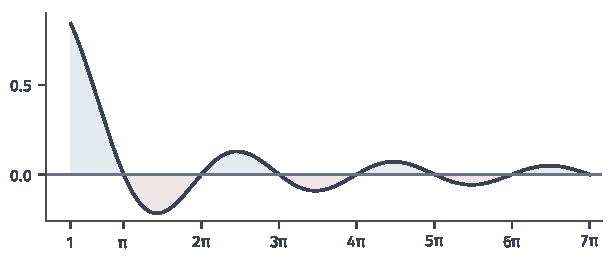
\includegraphics[width=104mm]{figures/04-spaces-measures-and-geometry/02-measure/matplotlib/integ-sinc-improper/figure.pdf}
  \caption{$f(x)=\sin x/x$在$[1,7\pi]$上的图像，正瓣蓝底、负瓣红底。第$k$瓣$[k\pi,(k+1)\pi]$上$\lvert f\rvert$的面积不小于$2/((k+1)\pi)$，各瓣面积之和按调和级数发散。按$x$增大的次序累加时正负瓣相互抵消，反常积分收敛。}
  \label{fig:integ-sinc-improper}
\end{BookInlineFigure}

图中正瓣与负瓣交替出现，面积按$1/k$缓慢减小。反常积分按从左到右的次序累加，正负瓣两两抵消，部分和收敛；把正瓣和负瓣分别累加，各自都发散。这与条件收敛的数项级数$\sum(-1)^k/k$相同：它的值依赖求和的次序。

测度积分不使用任何次序，所以它只接受与次序无关的绝对收敛情形。这并不是新积分的缺陷：需要条件收敛积分的场合，仍可以把它写成Lebesgue积分在截断区间上的极限。

\section{积分与极限}
\label{sec:integ-limits}

分析中的许多函数是逐步逼近得到的：级数的部分和、截断区间上的函数、越来越细的平均。若一列可测函数逐点趋于目标函数，我们希望各次积分也趋于目标函数的积分，这样就能用容易计算的近似求出难以直接计算的积分。本节先说明逐点与几乎处处收敛的含义，用一个尖峰例子说明交换不能无条件进行；再依次研究递增逼近、非负函数列的下极限估计，以及由同一个可积函数控制的函数列。收敛方式的系统比较以及一致可积性，留到第~\ref{chap:normed-spaces}章。

\subsection{逐点逼近与积分极限}
\label{sec:integ-pointwise}

\paragraph{逐点收敛与几乎处处收敛}
固定一个输入点$x$，函数列$f_1,f_2,\dots$在这一点的取值是一列数$f_1(x),f_2(x),\dots$。若对每个$x\in X$，这列数都收敛到$f(x)$，称$f_n$\term{逐点收敛}（pointwise convergence）到$f$。积分看不见零测集，所以只需要求收敛在零测集之外成立：若存在零测集$N$，使$f_n(x)\to f(x)$对每个$x\notin N$成立，称$f_n$\term{几乎处处收敛}（almost everywhere convergence）到$f$。

几乎处处的极限只确定到零测集。若$f_n$几乎处处收敛到$f$与$g$，两个例外集之并仍是零测集，在它之外$f=g$，所以$f=g$几乎处处成立。极限函数的可测性也要留意：收敛点集$\{x:\limsup_nf_n(x)=\liminf_nf_n(x)\}$可测，在其上取$\limsup_nf_n$、其外取$0$，就得到一个可测的极限代表；在完备测度空间中，任何几乎处处等于它的函数都可测。下面谈到几乎处处收敛的极限时，总指这样一个可测代表。

\paragraph{积分不随逐点极限收敛的例子}
在$[0,1]$上取
\[
 f_n(x)=n\mathbf 1_{(0,1/n)}(x),\qquad n\geq1.
\]
对$x=0$，每个$f_n(0)=0$；对$x>0$，当$n>1/x$时$x\notin(0,1/n)$，$f_n(x)=0$。所以$f_n$逐点收敛到$0$。但每个$f_n$是高为$n$、宽为$1/n$的矩形，$\int f_n=1$，于是
\[
 \lim_{n\to\infty}\int_{[0,1]}f_n\,\mathrm d\lambda=1\neq0=\int_{[0,1]}\lim_{n\to\infty}f_n\,\mathrm d\lambda .
\]
质量没有消失，而是挤进了越来越窄的区间：每一点最终都看不到尖峰，尖峰的面积却始终是$1$。这说明积分与极限的交换需要条件。下面三小节给出三种条件：函数列递增，函数列非负（只得到单向估计），以及函数列被一个可积函数共同控制。

\subsection{单调收敛}
\label{sec:integ-monotone-convergence}

\paragraph{单调收敛定理}
尖峰例子中的函数列不单调：$f_n$在$(0,1/n)$上增大，在别处变为零。若函数列递增，质量只会不断加入，不会挤走，积分就能与极限交换。引理~\ref{lem:integ-increasing-simple}对递增的简单函数列证明了这一点，同样的论证对一般的递增可测函数列成立。

\begin{theorem}[单调收敛定理]
\label{thm:integ-monotone-convergence}
设$f_n:X\to[0,+\infty]$可测，$f_1\leq f_2\leq\cdots$几乎处处成立，$f=\lim_nf_n$几乎处处成立。则
\[
 \int_Xf\,\mathrm d\mu=\lim_{n\to\infty}\int_Xf_n\,\mathrm d\mu,
\]
两边在$[0,+\infty]$中相等。
\end{theorem}

\begin{proof}
把可数个例外零测集合并为$N$，在$N$上把$f$与全部$f_n$改为$0$，积分都不变，所以不妨设单调性与收敛处处成立。由单调性，$\int f_n$递增且不超过$\int f$，极限存在且不超过$\int f$。

反方向，任取简单函数$0\leq s\leq f$与$c\in(0,1)$，令$E_n=\{f_n\geq cs\}$。它们可测且递增；与引理~\ref{lem:integ-increasing-simple}的证明相同，$s(x)>0$时$f(x)>cs(x)$，所以$\bigcup_nE_n=X$。于是$\int f_n\geq c\int s\mathbf 1_{E_n}\to c\int s$。令$c\uparrow1$，再对$s$取上确界，得$\lim_n\int f_n\geq\int f$。
\end{proof}

积分值允许为$+\infty$：若$\int f=+\infty$，定理说$\int f_n\to+\infty$。非负性也不能省去，否则会遇到$\int f_1=-\infty$这样无法向上逼近的起点；只要$f_1$可积，对$f_n-f_1$应用定理即可处理取负值的递增列。

\paragraph{非负级数与可数区域}
递增列最常见的来源是非负项的部分和与逐步扩大的区域。设$g_k\geq0$可测，部分和$\sum_{k\leq n}g_k$递增到$\sum_kg_k$，由单调收敛定理与有限可加性，
\begin{equation}
 \int\sum_{k=1}^\infty g_k\,\mathrm d\mu=\sum_{k=1}^\infty\int g_k\,\mathrm d\mu .
 \label{eq:integ-series-termwise}
\end{equation}
非负函数项级数总可以逐项积分，两边允许为$+\infty$。取$g_k=f\mathbf 1_{A_k}$，其中$A_k$两两不交，就得到第~\ref{sec:integ-domain-additivity}小节预告的可数区域分解$\int_{\bigcup_kA_k}f=\sum_k\int_{A_k}f$；所以对非负可测的$f$，$A\mapsto\int_Af\,\mathrm d\mu$是测度。

两个计算说明式~\eqref{eq:integ-series-termwise}的用法。在$\mathbb N$上取计数测度，非负函数$f=\sum_nf(n)\mathbf 1_{\{n\}}$，逐项积分得$\int f=\sum_nf(n)$：离散空间上的非负积分就是级数求和。在$[0,1)$上，$-\log(1-x)=\sum_{n\geq1}x^n/n$各项非负，逐项积分并用定理~\ref{thm:integ-riemann-lebesgue}计算多项式的积分，得
\[
 \int_{[0,1)}-\log(1-x)\,\mathrm dx=\sum_{n\geq1}\frac1{n(n+1)}=\sum_{n\geq1}\Bigl(\frac1n-\frac1{n+1}\Bigr)=1 .
\]

\paragraph{反常积分定理的证明}
现在补上第~\ref{sec:integ-improper}小节的依据。

\begin{proof}[定理~\ref{thm:integ-improper}的证明]
取$b_n\uparrow\beta$。由定理~\ref{thm:integ-riemann-lebesgue}，每个$f\mathbf 1_{[a,b_n]}$关于$\mathcal L$可测，它们逐点收敛到$f\mathbf 1_I$，所以$f$在$I$上可测。

第1条：$f\geq0$时$f\mathbf 1_{[a,b_n]}$递增到$f\mathbf 1_I$，单调收敛定理与定理~\ref{thm:integ-riemann-lebesgue}给出$\int_If\,\mathrm d\lambda=\lim_n\int_a^{b_n}f\,\mathrm dx$。由于$b\mapsto\int_a^bf$递增，沿任意$b_n\uparrow\beta$的极限都等于$b\uparrow\beta$时的极限。

第2条：$\lvert f\rvert$在每个$[a,b]$上黎曼可积（它的振幅不超过$f$的振幅），由第1条$\int_I\lvert f\rvert\,\mathrm d\lambda=\lim_{b\uparrow\beta}\int_a^b\lvert f\rvert$，可积性的等价随之成立。可积时$f^\pm=\frac12(\lvert f\rvert\pm f)$也在每个$[a,b]$上黎曼可积，由第1条$\int_If^\pm\,\mathrm d\lambda=\lim_b\int_a^bf^\pm$，两个极限都有限，相减即得。
\end{proof}

\subsection{Fatou估计}
\label{sec:integ-fatou}

\paragraph{下极限的积分}
对不单调的非负函数列，尖峰例子说明等式可以失败。但失败只有一个方向：极限函数的积分不会\emph{超过}积分的极限，因为非负函数的质量只能在极限中丢失，不能凭空产生。把不单调的列换成它的尾部下确界，就得到一个递增列，可以用单调收敛定理。

\begin{theorem}[Fatou引理]
\label{thm:integ-fatou}
设$f_n:X\to[0,+\infty]$可测。则
\[
 \int_X\liminf_{n\to\infty}f_n\,\mathrm d\mu\leq\liminf_{n\to\infty}\int_Xf_n\,\mathrm d\mu .
\]
\end{theorem}

\begin{proof}
令$g_n=\inf_{k\geq n}f_k$。它们是非负可测函数，关于$n$递增，极限为$\liminf_nf_n$。由单调收敛定理，$\int\liminf_nf_n=\lim_n\int g_n$。又对每个$k\geq n$有$g_n\leq f_k$，所以$\int g_n\leq\inf_{k\geq n}\int f_k$。令$n\to\infty$，右边趋于$\liminf_n\int f_n$。
\end{proof}

\paragraph{严格不等与单向性}
在尖峰例子中，$\liminf_nf_n=0$，左边为$0$，右边为$1$，不等式严格成立。所以Fatou引理一般只给出单向估计：当我们知道$\int f_n$有界时，它保证极限函数可积，并给出积分的上界，却不给出积分的值。

非负性不能省去。把尖峰换成$-f_n=-n\mathbf 1_{(0,1/n)}$，下极限仍为$0$，左边为$0$，右边为$-1$，不等式反向。这说明Fatou引理依赖的是“质量只会丢失”这一非负性质。对取正负值的函数列，若有一个可积函数从下方控制它，可以先加上这个函数再用Fatou引理，下一小节正是这样做的。

\subsection{支配收敛}
\label{sec:integ-dominated-convergence}

\paragraph{支配收敛定理}
尖峰的质量能够逃逸，是因为$f_n$的高度没有共同的可积上界。若所有$f_n$都被同一个可积函数压住，质量就无处可逃：它不能挤进越来越窄的区间无限升高，也不能向无穷远处流走。

\begin{theorem}[支配收敛定理]
\label{thm:integ-dominated-convergence}
设$f_n$是实值或复值可测函数，$f_n\to f$几乎处处成立，并且存在可积函数$g\geq0$，使对每个$n$都有$\lvert f_n\rvert\leq g$几乎处处成立。则$f$可积，
\[
 \lim_{n\to\infty}\int_X\lvert f_n-f\rvert\,\mathrm d\mu=0,\qquad \lim_{n\to\infty}\int_Xf_n\,\mathrm d\mu=\int_Xf\,\mathrm d\mu .
\]
\end{theorem}

\begin{proof}
合并可数个例外零测集，不妨设收敛与控制处处成立。先设$f_n$实值。由$\lvert f_n\rvert\leq g$取极限得$\lvert f\rvert\leq g$，所以$f$可积。令$h_n=2g-\lvert f_n-f\rvert$，由$\lvert f_n-f\rvert\leq\lvert f_n\rvert+\lvert f\rvert\leq2g$知$h_n\geq0$，且$h_n\to2g$。由Fatou引理，
\[
 \int2g\leq\liminf_n\int\bigl(2g-\lvert f_n-f\rvert\bigr)=\int2g-\limsup_n\int\lvert f_n-f\rvert,
\]
其中等号用了线性性，$\int2g$有限，可以从两边消去，得$\limsup_n\int\lvert f_n-f\rvert\leq0$。再由绝对值估计$\lvert\int f_n-\int f\rvert\leq\int\lvert f_n-f\rvert\to0$。

复值情形，记$f_n=u_n+\mathrm iv_n$。$\lvert u_n\rvert,\lvert v_n\rvert\leq\lvert f_n\rvert\leq g$，实部与虚部分别几乎处处收敛，由实值情形分别交换极限与积分；误差$\int\lvert f_n-f\rvert\leq\int\lvert u_n-u\rvert+\int\lvert v_n-v\rvert\to0$。
\end{proof}

结论$\int\lvert f_n-f\rvert\to0$比积分值收敛更强：它说的是近似函数整体上接近目标，而不仅是总量接近。由上一节的误差控制，它对每个可测子集$A$同时给出$\lvert\int_Af_n-\int_Af\rvert\leq\int\lvert f_n-f\rvert\to0$。

\paragraph{共同上界的作用}
图~\ref{fig:integ-dominating-envelope}对照了一个可控与一个不可控的例子。在$[0,1]$上$f_n(x)=x^n$逐点收敛到$\mathbf 1_{\{1\}}$，几乎处处为零，所有$f_n$都被常数$1$控制，常数在$[0,1]$上可积，所以$\int x^n=1/(n+1)\to0$，与支配收敛一致。

尖峰列$f_n=n\mathbf 1_{(0,1/n)}$没有可积的控制函数。任何控制函数都不小于上包络$h=\sup_nf_n$，而$h$在$[\frac1{n+1},\frac1n)$上等于$n$，于是$h(x)\geq1/x-1$，后者在$(0,1)$上积分为$+\infty$。这正是积分极限失败的原因：共同上界缺失时，质量可以集中到越来越小的集合上。

\begin{figure}[!htbp]
 \centering
 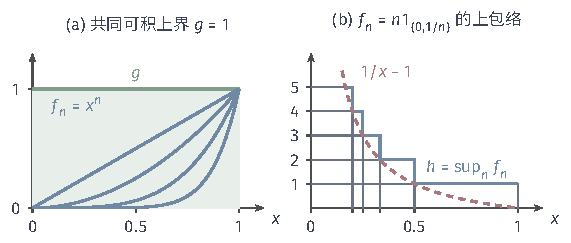
\includegraphics[width=96.633mm]{figures/02-abstract-mathematics/01-metric-and-measure/tikz/c3-dominating-envelope/figure.pdf}
 \caption{控制函数与上包络。(a)$[0,1]$上$f_n=x^n$（$n=1,2,4,8$）都位于可积函数$g=1$之下，积分$1/(n+1)\to0$。(b)$f_n=n\mathbf 1_{(0,1/n)}$（灰色，$n=1,\dots,5$）积分恒为$1$；上包络$h=\sup_nf_n$（蓝色阶梯）在$[\frac1{n+1},\frac1n)$上等于$n$，不小于$1/x-1$（红色虚线），后者在$(0,1)$上积分为$+\infty$，所以不存在可积的控制函数。}
 \label{fig:integ-dominating-envelope}
\end{figure}

支配条件是充分而非必要的：有些函数列没有可积的共同上界，积分仍然收敛。刻画积分收敛的确切条件需要一致可积性，它与依测度收敛等收敛方式一起在第~\ref{chap:normed-spaces}章讨论。在有限测度空间上，最常用的特例是：一致有界且几乎处处收敛的函数列，以常数为控制函数，积分可以与极限交换。

\section{累次积分}
\label{sec:integ-iterated}

计算平面区域上的累计时，我们习惯先沿一个方向积分，再沿另一个方向积分；计算双重级数时，先按行求和再把行和相加。这些做法都把一个联合累计拆成依次累计，并默认两种次序给出同一个结果。

有限矩阵的元素求和可以先行后列，也可以先列后行，这是有限加法的交换律。无穷的情形则需要条件，本节后面会给出一个无穷矩阵，两种次序的结果不同。下面先为两个测度空间的乘积建立集合族和乘积测度，再分别对非负函数与绝对可积函数证明这种拆分与换序成立。

\subsection{乘积测度}
\label{sec:integ-product-measure}

\paragraph{可测矩形与乘积$\sigma$代数}
设$(X,\mathcal A,\mu)$与$(Y,\mathcal B,\nu)$是测度空间。在$X\times Y$上，最简单的集合是$A\times B$，其中$A\in\mathcal A$、$B\in\mathcal B$，称为\term{可测矩形}（measurable rectangle）。它的“面积”应当是$\mu(A)\nu(B)$。可测矩形的有限并一般不再是矩形，所以要像上一章那样由它们生成$\sigma$代数。

\begin{definition}[乘积$\sigma$代数]
\label{def:integ-product-sigma}
由全体可测矩形生成的$\sigma$代数称为\term{乘积$\sigma$代数}（product sigma-algebra），记作$\mathcal A\otimes\mathcal B$。
\end{definition}

可测矩形的“边”可以是任意可测集，不必是区间。图~\ref{fig:integ-product-rectangles}(a)中$A$由两段组成，$A\times B$也就由两块组成，面积仍是$\lambda(A)\lambda(B)=1.8\times1=1.8$。

两个可测矩形之交仍是可测矩形：
\[
 (A\times B)\cap(A'\times B')=(A\cap A')\times(B\cap B').
\]
所以可测矩形构成$\pi$系统，后面的唯一性论证要用到这一点。

\begin{BookInlineFigure}
  \centering
  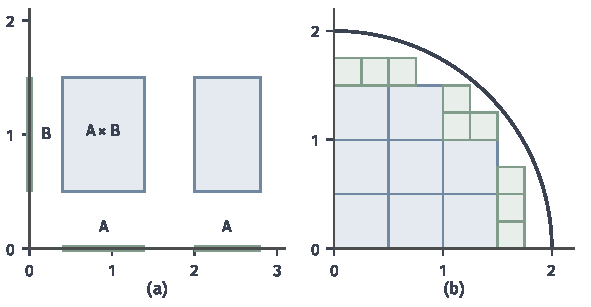
\includegraphics[width=100mm]{figures/04-spaces-measures-and-geometry/02-measure/matplotlib/integ-product-rectangles/figure.pdf}
  \caption{乘积可测结构由矩形生成。(a)取$A=[0.4,1.4]\cup[2.0,2.8]$、$B=[0.5,1.5]$，可测矩形$A\times B$由两块组成，绿色线段分别是$A$与$B$。(b)半径为$2$的四分之一圆盘不是矩形，蓝色矩形是边长$0.5$的网格中完全落在圆盘内的方格，绿色矩形是边长$0.25$的网格补充的方格；逐层加细的矩形不交并从内部逼近圆盘。}
  \label{fig:integ-product-rectangles}
\end{BookInlineFigure}

在欧氏空间上，乘积$\sigma$代数就是Borel代数：
\begin{equation}
 \mathcal B(\mathbb R)\otimes\mathcal B(\mathbb R)=\mathcal B(\mathbb R^2).
 \label{eq:integ-borel-product}
\end{equation}
一方面，开集是可数个有理顶点开矩形之并，开矩形是可测矩形，如图~\ref{fig:integ-product-rectangles}(b)所示，所以Borel集都在乘积$\sigma$代数中。另一方面，$A\times\mathbb R$是$A$在连续投影下的原像，对Borel集$A$是Borel集；$A\times B$是这样两个集合之交，也是Borel集。

\paragraph{截面}
依次累计的第一步是固定一个坐标。对$E\subseteq X\times Y$与$x\in X$，称$E_x=\{y\in Y:(x,y)\in E\}$为$E$在$x$处的\term{截面}（section）；类似地，$E^y=\{x\in X:(x,y)\in E\}$。对函数$f$，固定$x$得到截面函数$f_x(y)=f(x,y)$，固定$y$得到$f^y(x)=f(x,y)$。

截面的形状取决于固定哪个坐标。圆环在靠近中心的$x$处的截面是两段区间，在靠外的$x$处则是一段。下面先确认截面总是可测的，否则内层积分无从谈起。

\begin{lemma}[截面的可测性]
\label{lem:integ-section-measurable}
若$E\in\mathcal A\otimes\mathcal B$，则对每个$x$有$E_x\in\mathcal B$，对每个$y$有$E^y\in\mathcal A$。若$f$是$\mathcal A\otimes\mathcal B$可测函数，则每个$f_x$是$\mathcal B$可测的，每个$f^y$是$\mathcal A$可测的。
\end{lemma}

\begin{proof}
固定$x$，令$\mathcal E$为满足$E_x\in\mathcal B$的集合$E\subseteq X\times Y$全体。截面与补集、可数并可交换：
\[
 (X\times Y\setminus E)_x=Y\setminus E_x,\qquad\Bigl(\bigcup_nE_n\Bigr)_x=\bigcup_n(E_n)_x .
\]
所以$\mathcal E$是$\sigma$代数。对可测矩形，$(A\times B)_x$在$x\in A$时为$B$、否则为空集，所以$\mathcal E$含全部可测矩形，从而含$\mathcal A\otimes\mathcal B$。函数的情形由$\{f_x>a\}=(\{f>a\})_x$得到。$y$一侧对称。
\end{proof}

\paragraph{截面测度的可测性}
乘积测度的候选定义是沿$x$累计截面的测度，这相当于把区域切成薄片，每片的“长度”乘以厚度再相加：
\[
 E\mapsto\int_X\nu(E_x)\,\mathrm d\mu(x).
\]
为此要先知道$x\mapsto\nu(E_x)$可测。这一步需要$\sigma$有限条件。

\begin{lemma}[截面测度的可测性]
\label{lem:integ-section-measure}
设$\nu$是$\sigma$有限测度，$E\in\mathcal A\otimes\mathcal B$。则$x\mapsto\nu(E_x)$是$X$上的可测函数。
\end{lemma}

\begin{proof}
先设$\nu$有限。令$\mathcal D$为使$x\mapsto\nu(E_x)$可测的$E\in\mathcal A\otimes\mathcal B$全体。对可测矩形，$\nu((A\times B)_x)=\nu(B)\mathbf 1_A(x)$，可测，所以$\mathcal D$含可测矩形这一$\pi$系统。

$\mathcal D$是$\lambda$系统，逐条核对。全集$X\times Y$的截面测度是常数$\nu(Y)$。补集的截面测度为$\nu(Y)-\nu(E_x)$，这里用到$\nu$有限，差才有意义。不交可数并的截面测度是各截面测度之和，可测函数的可数和可测。由$\pi$--$\lambda$定理，$\mathcal D=\mathcal A\otimes\mathcal B$。

一般情形取$Y_m\in\mathcal B$两两不交、并为$Y$且$\nu(Y_m)<+\infty$，令$\nu_m(B)=\nu(B\cap Y_m)$。每个$\nu_m$有限，由上一段$x\mapsto\nu_m(E_x)$可测，而$\nu(E_x)=\sum_m\nu_m(E_x)$是可数个可测函数之和。
\end{proof}

\paragraph{乘积测度的构造}
截面测度可测以后，沿$x$累计截面测度就得到一个候选的乘积测度；沿$y$累计得到另一个候选。下面的定理说明二者是同一个测度，并且它由矩形上的取值唯一确定。

\begin{theorem}[乘积测度的存在唯一性]
\label{thm:integ-product-measure}
设$\mu,\nu$都是$\sigma$有限测度。则$\mathcal A\otimes\mathcal B$上存在唯一的测度$\pi$，使
\begin{equation}
 \pi(A\times B)=\mu(A)\nu(B),\qquad A\in\mathcal A,\ B\in\mathcal B,
 \label{eq:integ-product-rectangle}
\end{equation}
并且对每个$E\in\mathcal A\otimes\mathcal B$，
\begin{equation}
 \pi(E)=\int_X\nu(E_x)\,\mathrm d\mu(x)=\int_Y\mu(E^y)\,\mathrm d\nu(y).
 \label{eq:integ-product-sections}
\end{equation}
\end{theorem}

\begin{proof}
令$\pi_1(E)=\int_X\nu(E_x)\,\mathrm d\mu(x)$，由引理~\ref{lem:integ-section-measure}，被积函数非负可测。空集的截面都是空集，所以$\pi_1(\varnothing)=0$。若$E_n$两两不交，各截面$(E_n)_x$也两两不交，于是$\nu((\bigcup_nE_n)_x)=\sum_n\nu((E_n)_x)$。对$x$积分并用式~\eqref{eq:integ-series-termwise}逐项积分，得到
\[
 \pi_1\Bigl(\bigcup_nE_n\Bigr)=\sum_n\pi_1(E_n).
\]
所以$\pi_1$是测度。对矩形，
\[
 \pi_1(A\times B)=\int_X\nu(B)\mathbf 1_A\,\mathrm d\mu=\mu(A)\nu(B).
\]
同理$\pi_2(E)=\int_Y\mu(E^y)\,\mathrm d\nu(y)$也是满足式~\eqref{eq:integ-product-rectangle}的测度。

唯一性。取$X_n\in\mathcal A$、$Y_m\in\mathcal B$分别覆盖$X$、$Y$且测度有限，可数个矩形$X_n\times Y_m$覆盖$X\times Y$，在任何满足式~\eqref{eq:integ-product-rectangle}的测度下都取有限值。两个这样的测度在可测矩形这一$\pi$系统上相等，由第~\ref{chap:measure}章生成$\pi$系统上的唯一性定理，它们在$\mathcal A\otimes\mathcal B$上相等。特别地$\pi_1=\pi_2$，这就是式~\eqref{eq:integ-product-sections}。
\end{proof}

\begin{definition}[乘积测度]
\label{def:integ-product-measure}
定理~\ref{thm:integ-product-measure}中的测度称为$\mu$与$\nu$的\term{乘积测度}（product measure），记作$\mu\otimes\nu$。
\end{definition}

下面在一个可以逐项计算的网格上验证式~\eqref{eq:integ-product-sections}。两种切法分别相当于先按行、先按列累计，结果相同正是这个公式的含义。

\begin{example}[有限网格上的乘积测度]
\label{ex:integ-product-grid}
取$X=\{1,2\}$，质量为$\mu(\{1\})=1$、$\mu(\{2\})=2$；取$Y=\{a,b,c\}$，质量为$\nu(\{a\})=1$、$\nu(\{b\})=3$、$\nu(\{c\})=1$。乘积测度给格点$(i,y)$的质量$\mu(\{i\})\nu(\{y\})$。取
\[
 E=\{(1,a),(1,b),(2,b),(2,c)\}.
\]
按$x$切，两个截面的$\nu$测度为
\[
 \nu(E_1)=1+3=4,\qquad\nu(E_2)=3+1=4,
\]
于是
\[
 \int\nu(E_x)\,\mathrm d\mu=1\cdot4+2\cdot4=12 .
\]

按$y$切，三个截面的$\mu$测度为
\[
 \mu(E^a)=1,\qquad\mu(E^b)=1+2=3,\qquad\mu(E^c)=2,
\]
于是
\[
 \int\mu(E^y)\,\mathrm d\nu=1\cdot1+3\cdot3+1\cdot2=12 .
\]
两种切法得到同一个数。
\end{example}

\paragraph{与Lebesgue测度的关系}
在$\mathbb R^2$上，$\lambda\otimes\lambda$与第~\ref{chap:measure}章的二维Lebesgue测度$\lambda_2$都定义在式~\eqref{eq:integ-borel-product}的$\sigma$代数上，在左开右闭矩形上都等于边长之积；由唯一性它们相等。归纳可得$\lambda_d$等于$d$个$\lambda$的乘积。于是$\mathbb R^d$上Borel函数的积分可以逐个坐标计算，这是下面两个定理的主要用途。

\paragraph{乘积集合族与完备化}
乘积$\sigma$代数与测度的完备化是两回事。即使$\mu,\nu$都完备，$\mathcal A\otimes\mathcal B$也未必完备。取$\mathcal L$为Lebesgue可测集，$S\subseteq\mathbb R$不Lebesgue可测，$E=S\times\{0\}$。$E$含于$\mathbb R\times\{0\}$，后者的$\lambda\otimes\lambda$测度为$0$，所以$E$属于完备化；但截面$E^0=S$不可测，由引理~\ref{lem:integ-section-measurable}，$E\notin\mathcal L\otimes\mathcal L$。

二维Lebesgue可测集是$\lambda_2$的完备化，它比$\mathcal L\otimes\mathcal L$大。所以在完备化的乘积测度下，不能默认每个截面都可测；下面的定理会把这种例外限制在零测的参数集上。

\subsection{Tonelli定理}
\label{sec:integ-tonelli}

\paragraph{非负函数的换序}
式~\eqref{eq:integ-product-sections}说的是指示函数的联合积分等于两种次序的累次积分。对一般的非负函数，沿积分的构造步骤推广：指示函数、简单函数、递增极限。非负贡献不会相互抵消，所以结论允许各方都等于$+\infty$。先对一个变量积分、再对另一个变量积分所得的量称为\term{累次积分}（iterated integral）。

\begin{theorem}[Tonelli定理]
\label{thm:integ-tonelli}
设$\mu,\nu$都是$\sigma$有限测度，$f:X\times Y\to[0,+\infty]$是$\mathcal A\otimes\mathcal B$可测函数。则$x\mapsto\int_Yf_x\,\mathrm d\nu$与$y\mapsto\int_Xf^y\,\mathrm d\mu$分别可测，并且下面三者在$[0,+\infty]$中相等：
\begin{equation}
\begin{aligned}
 \int_{X\times Y}f\,\mathrm d(\mu\otimes\nu)&=\int_X\Bigl(\int_Yf(x,y)\,\mathrm d\nu(y)\Bigr)\mathrm d\mu(x)\\
 &=\int_Y\Bigl(\int_Xf(x,y)\,\mathrm d\mu(x)\Bigr)\mathrm d\nu(y).
\end{aligned}
 \label{eq:integ-tonelli}
\end{equation}
\end{theorem}

\begin{proof}
由引理~\ref{lem:integ-section-measurable}，各截面函数可测，内层积分有意义。证明按函数的构造分三步，只写$x$先固定的一侧，另一侧对称。

第一步，$f=\mathbf 1_E$，$E\in\mathcal A\otimes\mathcal B$。内层积分是$\nu(E_x)$，由引理~\ref{lem:integ-section-measure}可测，外层积分等于$(\mu\otimes\nu)(E)$，这就是式~\eqref{eq:integ-product-sections}。

第二步，$f$是非负简单函数，即有限个$c_i\mathbf 1_{E_i}$之和。内层积分是相应$c_i\nu((E_i)_x)$之和，可测，由线性性逐项得到式~\eqref{eq:integ-tonelli}。

第三步，一般的$f$。取二进分层逼近$\varphi_n\uparrow f$，每个$\varphi_n$是$\mathcal A\otimes\mathcal B$可测的简单函数。对每个$x$，$(\varphi_n)_x\uparrow f_x$，由单调收敛定理，
\[
 \int_Y(\varphi_n)_x\,\mathrm d\nu\uparrow\int_Yf_x\,\mathrm d\nu .
\]
作为可测函数的递增极限，$x\mapsto\int f_x\,\mathrm d\nu$可测。再对$x$用一次单调收敛定理，并在乘积空间上对$\varphi_n\uparrow f$用一次，由第二步的等式取极限即得。
\end{proof}

换序的实际用处是：内层积分按一种次序算不出来，换一种次序就能算。下面的例子中，$e^{y^2}$没有初等原函数，先对$y$积分行不通，先对$x$积分却只是乘以区间长度。

\begin{example}[换序计算]
\label{ex:integ-tonelli-swap}
计算累次积分
\[
 I=\int_0^1\Bigl(\int_x^1e^{y^2}\,\mathrm dy\Bigr)\mathrm dx .
\]
被积函数$f(x,y)=e^{y^2}\mathbf 1_{\{0\leq x\leq y\leq1\}}$非负且Borel可测，由Tonelli定理可以换序。固定$y$，$x$的截面是$[0,y]$，于是
\[
 I=\int_0^1\Bigl(\int_0^ye^{y^2}\,\mathrm dx\Bigr)\mathrm dy=\int_0^1ye^{y^2}\,\mathrm dy .
\]
令$w=y^2$，$\mathrm dw=2y\,\mathrm dy$，得到
\[
 I=\frac12\int_0^1e^w\,\mathrm dw=\frac{e-1}2 .
\]
换序之所以合法，只因为被积函数非负，不需要事先知道积分有限。
\end{example}

图~\ref{fig:integ-section-swap}画出了这个例子的积分区域。同一个三角形，竖着切时每个截面从对角线走到顶边，横着切时每个截面从左边走到对角线；换序就是把这两种切片方式互换，新的积分限要从图上读出来。

\begin{BookInlineFigure}
  \centering
  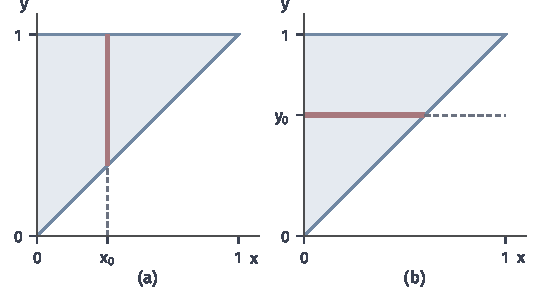
\includegraphics[width=92mm]{figures/04-spaces-measures-and-geometry/02-measure/matplotlib/integ-section-swap/figure.pdf}
  \caption{三角形$T=\{0\leq x\leq y\leq1\}$的两种截面。(a)固定$x=x_0$，红色线段是$y\in[x_0,1]$。(b)固定$y=y_0$，红色线段是$x\in[0,y_0]$，虚线部分不在$T$内。}
  \label{fig:integ-section-swap}
\end{BookInlineFigure}

\paragraph{完备化下的Tonelli定理}
若$f$只对完备化的乘积测度可测，截面函数可能不可测，结论要改成“几乎所有参数”。设$\mu,\nu$完备且$\sigma$有限，$f\geq0$对$\mu\otimes\nu$的完备化可测。

第一步找一个可测的替身。存在$\mathcal A\otimes\mathcal B$可测的$g\geq0$与$\mu\otimes\nu$零测集$N\in\mathcal A\otimes\mathcal B$，使$f=g$在$N$外成立：对指示函数，这就是完备化的定义（可测集等于乘积可测集并上零测集的子集），再经简单函数的递增逼近推广到一般的$f$。

第二步把零测的影响限制在参数上。由式~\eqref{eq:integ-product-sections}，$\int\nu(N_x)\,\mathrm d\mu=0$，所以对几乎每个$x$，$N_x$是$\nu$零测集。在这些$x$处，$f_x$与可测的$g_x$只在零测集上不同，由$\nu$的完备性可测，且积分相同。

对$g$用Tonelli定理，就得到式~\eqref{eq:integ-tonelli}，只是内层积分只对几乎每个$x$有定义，在例外的零测集上可以任意取值。$\mathbb R^d$上Lebesgue可测函数的累次积分正是这种情形。

\paragraph{$\sigma$有限条件}
$\sigma$有限条件不能省去。在$X=Y=[0,1]$上取$\mu$为Lebesgue测度，$\nu$为以全部Borel集为可测范围的计数测度，它不是$\sigma$有限的。对角线$D=\{(x,x):x\in[0,1]\}$是闭集，属于$\mathcal B([0,1])\otimes\mathcal B([0,1])$。

每个$x$截面$D_x=\{x\}$的计数为$1$，每个$y$截面$D^y=\{y\}$的Lebesgue测度为$0$，于是
\[
 \int_X\nu(D_x)\,\mathrm d\mu(x)=1,\qquad \int_Y\mu(D^y)\,\mathrm d\nu(y)=0 .
\]
两种次序不相等，式~\eqref{eq:integ-product-sections}失效。乘积测度构造中的唯一性论证正是在这里失去了依据：计数测度没有有限质量的覆盖片。

\paragraph{非负双重级数}
取两个$\mathbb N$上的计数测度，非负函数$a(m,n)=a_{m,n}$对乘积$\sigma$代数$\mathcal P(\mathbb N\times\mathbb N)$可测，乘积测度是$\mathbb N\times\mathbb N$上的计数测度。Tonelli定理给出
\[
 \sum_m\sum_na_{m,n}=\sum_n\sum_ma_{m,n},
\]
两边可以为$+\infty$：非负双重级数总可以交换求和次序。下一小节将看到，有正有负的双重级数并非如此。

\subsection{Fubini定理}
\label{sec:integ-fubini}

\paragraph{绝对可积函数的换序}
对取正负值或复值的函数，正负贡献的抵消可能依赖求和或积分的次序。解决办法是先对$\lvert f\rvert$用Tonelli定理核对绝对可积性，有了这一保证，再把$f$拆成正负部分或实部虚部，分别使用Tonelli定理。

\begin{theorem}[Fubini定理]
\label{thm:integ-fubini}
设$\mu,\nu$都是$\sigma$有限测度，$f$是$X\times Y$上$\mathcal A\otimes\mathcal B$可测的实值或复值函数，且
\begin{equation}
 \int_X\Bigl(\int_Y\lvert f(x,y)\rvert\,\mathrm d\nu(y)\Bigr)\mathrm d\mu(x)<+\infty .
 \label{eq:integ-fubini-condition}
\end{equation}
则$f$关于$\mu\otimes\nu$可积，并且：
\begin{enumerate}
 \item 对$\mu$-几乎每个$x$，$f_x$关于$\nu$可积；对$\nu$-几乎每个$y$，$f^y$关于$\mu$可积。
 \item 令$F(x)=\int_Yf_x\,\mathrm d\nu$，在$f_x$不可积的例外集上令$F(x)=0$，则$F$关于$\mu$可积；对$y$同样定义的$G$关于$\nu$可积。
 \item 三种累计相等：
 \begin{equation}
  \int_{X\times Y}f\,\mathrm d(\mu\otimes\nu)=\int_XF\,\mathrm d\mu=\int_YG\,\mathrm d\nu .
  \label{eq:integ-fubini}
 \end{equation}
\end{enumerate}
\end{theorem}

\begin{proof}
对$\lvert f\rvert$用Tonelli定理，式~\eqref{eq:integ-fubini-condition}的累次积分等于$\lvert f\rvert$在乘积空间上的积分，所以$f$可积。

令
\[
 N=\Bigl\{x:\ \int_Y\lvert f_x\rvert\,\mathrm d\nu=+\infty\Bigr\}.
\]
由Tonelli定理，它是可测集；又$x\mapsto\int\lvert f_x\rvert$的积分有限，由引理~\ref{lem:integ-null-sets}第2条，$\mu(N)=0$。这就是第1条。

先设$f$实值。$f^+$与$f^-$都是非负可测函数，由Tonelli定理，$x\mapsto\int f^\pm_x\,\mathrm d\nu$可测，积分分别等于$\int f^\pm\,\mathrm d(\mu\otimes\nu)$，都有限。在$N$外两者都有限，所以在$N$外有
\[
 F(x)=\int_Yf^+_x\,\mathrm d\nu-\int_Yf^-_x\,\mathrm d\nu .
\]
在$N$上$F=0$，所以$F$可测。对$F$积分，去掉零测集$N$不改变积分，得到
\[
\begin{aligned}
 \int_XF\,\mathrm d\mu&=\int_{X\setminus N}\Bigl(\int_Yf^+_x\,\mathrm d\nu\Bigr)\mathrm d\mu-\int_{X\setminus N}\Bigl(\int_Yf^-_x\,\mathrm d\nu\Bigr)\mathrm d\mu\\
 &=\int f^+\,\mathrm d(\mu\otimes\nu)-\int f^-\,\mathrm d(\mu\otimes\nu).
\end{aligned}
\]
右端就是$\int f\,\mathrm d(\mu\otimes\nu)$。$y$一侧对称。复值情形对实部与虚部分别使用实值结论，二者的例外集之并仍是零测集。
\end{proof}

截面只需几乎处处可积，这是由内层积分自身的性质决定的：对某个零测的$x$集合，$f_x$可能不可积，内层积分没有定义。把这些点上的$F$统一取零，得到的是一个可测的外层被积函数，而外层积分看不见零测集上的取值。若改用完备化的乘积测度，再结合上一小节的完备化讨论，结论同样成立，只是截面可测性本身也只对几乎每个参数成立。

\paragraph{缺少绝对可积时的反例}
绝对可积的假设不能去掉。考虑$\mathbb N\times\mathbb N$上的计数测度与下面的无穷矩阵，图~\ref{fig:integ-fubini-counterexample}画出了它的左上角：
\[
 a_{i,j}=\begin{cases}1,&j=i,\\-1,&j=i+1,\\0,&\text{其他}.\end{cases}
\]

先按行累计。每一行只有$+1$与$-1$两个非零元，行和为$0$，所以
\[
 \sum_i\sum_ja_{i,j}=0 .
\]
再按列累计。第一列只有$a_{1,1}=1$，列和为$1$；第$j\geq2$列有$a_{j,j}=1$与$a_{j-1,j}=-1$，列和为$0$，所以
\[
 \sum_j\sum_ia_{i,j}=1 .
\]

\begin{BookInlineFigure}
  \centering
  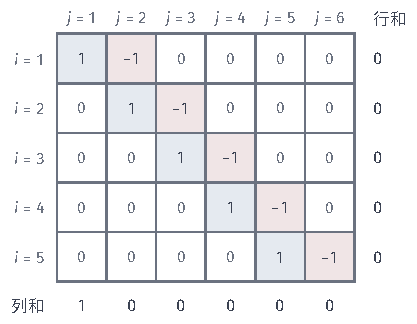
\includegraphics[width=70.672mm]{figures/04-spaces-measures-and-geometry/02-measure/tikz/integ-fubini-counterexample/figure.pdf}
  \caption{无穷矩阵$a_{i,j}$的左上角五行六列，矩阵向右下方继续。蓝色单元为$+1$，红色单元为$-1$。右侧是整行的和，下方是整列的和；第六列的$+1$位于第六行，在图外。}
  \label{fig:integ-fubini-counterexample}
\end{BookInlineFigure}

两种次序给出不同结果。原因是$\sum_{i,j}\lvert a_{i,j}\rvert=+\infty$，Fubini定理的条件不成立；每一行、每一列单独看都绝对可和，这并不够。这与有限矩阵不同：有限矩阵的两种次序总相同，因为有限和的重排不需要任何条件。

使用Fubini定理的标准步骤因此是：先对$\lvert f\rvert$任选一种方便的次序作累次积分，由Tonelli定理确认结果有限；然后才可以对$f$本身任意换序。对有界函数和有限测度，例如有界区域上的有界可测函数，第一步自动成立。

\section{微积分基本定理}
\label{sec:integ-ftc}

卷一的微积分基本定理有两个方向。被积函数$g$连续时，累计函数$G(x)=\int_a^xg(t)\,\mathrm dt$可导且$G'=g$；$F$连续可导时，$F(b)-F(a)=\int_a^bF'(t)\,\mathrm dt$。

有了Lebesgue积分，被积函数只需可积，导数也只需几乎处处存在，两个方向都要重新回答：可积函数的累计函数在什么意义下可导，导数是否回到被积函数？哪些函数能由几乎处处导数的积分恢复？本节在有界闭区间$[a,b]$上回答这两个问题，测度都是Lebesgue测度。

\subsection{变上限积分的导数}
\label{sec:integ-indefinite-derivative}

\paragraph{绝对连续函数}
先看什么样的函数有希望写成某个函数的累计。一致连续要求：区间足够短时，函数在两端的增量就小。要由导数恢复增量，这还不够。导数为零的点之间可能散布着许多极短的区间，函数恰好在这些区间上完成全部增长。需要控制的是许多互不相交的小区间上的\emph{总}增量。

\begin{definition}[绝对连续函数]
\label{def:integ-absolutely-continuous}
设$F:[a,b]\to\mathbb R$。若对任意$\varepsilon>0$存在$\delta>0$，使对$[a,b]$中任意有限个两两不交的开区间$(a_i,b_i)$（$i=1,\dots,m$），只要总长满足
\begin{equation}
 \sum_{i=1}^m(b_i-a_i)<\delta,
 \label{eq:integ-ac-length}
\end{equation}
就有
\begin{equation}
 \sum_{i=1}^m\lvert F(b_i)-F(a_i)\rvert<\varepsilon,
 \label{eq:integ-ac-increment}
\end{equation}
则称$F$为$[a,b]$上的\term{绝对连续函数}（absolutely continuous function）。
\end{definition}

取$m=1$就回到一致连续，所以绝对连续函数一致连续。区别在于$\delta$必须对任意多个小区间同时有效：区间个数不受限制，只限制总长度。图~\ref{fig:integ-absolute-continuity-intervals}中$F(x)=\sqrt x$，四段绿色区间总长$1.2$，对应的增量为
\[
 0.260,\qquad0.158,\qquad0.090,\qquad0.053,
\]
和约为$0.562$。绝对连续性要求，当总长趋于零时，增量之和也一致地趋于零，无论区间怎样分布、分成多少段。

\begin{BookInlineFigure}
  \centering
  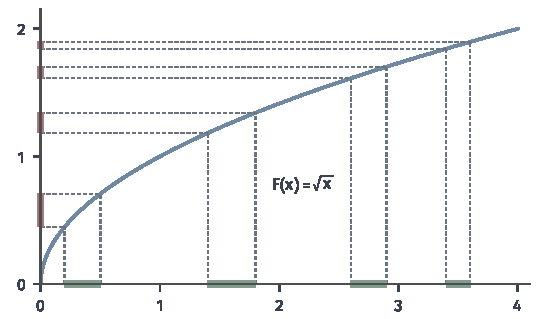
\includegraphics[width=92mm]{figures/04-spaces-measures-and-geometry/02-measure/matplotlib/integ-absolute-continuity-intervals/figure.pdf}
  \caption{绝对连续性控制的是多个不交区间上的总增量。$F(x)=\sqrt x$（蓝）。横轴上的绿色区间为$(0.2,0.5)$、$(1.4,1.8)$、$(2.6,2.9)$、$(3.4,3.6)$，纵轴上的红色线段是相应增量。靠近原点的区间虽短，增量却最大。}
  \label{fig:integ-absolute-continuity-intervals}
\end{BookInlineFigure}

若$F$满足Lipschitz条件$\lvert F(x)-F(y)\rvert\leq L\lvert x-y\rvert$，则总增量不超过$L$乘以总长度，取$\delta=\varepsilon/L$即可，所以Lipschitz函数绝对连续。$[a,b]$上连续可导的函数由中值定理满足Lipschitz条件，因而绝对连续。有限线性组合保持绝对连续，由三角不等式对各函数分别取$\delta$再取最小值即得。

这里的“绝对连续”描述函数增量受区间长度控制，与第~\ref{chap:measure-densities}章两个测度之间的绝对连续是不同的定义，两者的联系在那里说明。

\paragraph{变上限积分的绝对连续性}
设$g$在$[a,b]$上可积，令
\begin{equation}
 G(x)=\int_a^xg(t)\,\mathrm dt,\qquad a\leq x\leq b,
 \label{eq:integ-indefinite}
\end{equation}
称为$g$的\term{变上限积分}（indefinite integral）。多个不交区间上$G$的增量之和不超过$\lvert g\rvert$在这些区间之并上的积分，所以要证$G$绝对连续，需要的是：测度很小的集合上，$\lvert g\rvert$的积分也很小。

\begin{lemma}[积分的绝对连续性]
\label{lem:integ-small-sets}
设$g$关于$\mu$可积。则对任意$\varepsilon>0$存在$\delta>0$，使对每个满足$\mu(A)<\delta$的可测集$A$，都有$\int_A\lvert g\rvert\,\mathrm d\mu<\varepsilon$。
\end{lemma}

\begin{proof}
把$\lvert g\rvert$分成有界的截断$\min\{\lvert g\rvert,n\}$与尾部。截断随$n$递增到$\lvert g\rvert$，由单调收敛定理，$\int\min\{\lvert g\rvert,n\}\uparrow\int\lvert g\rvert<+\infty$。所以可取$n$使尾部满足
\[
 \int\bigl(\lvert g\rvert-\min\{\lvert g\rvert,n\}\bigr)\,\mathrm d\mu<\frac\varepsilon2 .
\]
令$\delta=\varepsilon/(2n)$。当$\mu(A)<\delta$时，截断部分不超过高度$n$乘以测度，于是
\[
 \int_A\lvert g\rvert\,\mathrm d\mu\leq\int_A\min\{\lvert g\rvert,n\}\,\mathrm d\mu+\frac\varepsilon2<n\delta+\frac\varepsilon2=\varepsilon .
\]
\end{proof}

对$[a,b]$中两两不交的$(a_i,b_i)$，令$A=\bigcup_i(a_i,b_i)$，由绝对值估计，
\[
 \sum_i\lvert G(b_i)-G(a_i)\rvert=\sum_i\Bigl\lvert\int_{a_i}^{b_i}g\Bigr\rvert\leq\int_A\lvert g\rvert\,\mathrm d\lambda .
\]
总长$\lambda(A)<\delta$时右侧小于$\varepsilon$，所以$G$绝对连续。例如在$[0,4]$上取$g(t)=1/(2\sqrt t)$，它在原点附近无界，但由反常积分定理$\int_0^xg=\sqrt x$，所以$\sqrt x$绝对连续；它在原点附近斜率无界，不是Lipschitz函数。

这里要区分两种对象。$g$只确定到零测集：在零测集上改动$g$，$G$完全不变。$G$却在每个点都有确定的值，并且是连续函数。所以下面关于$G'$的结论只能是“几乎处处等于$g$”，不能期望在每一点成立。

\paragraph{Vitali覆盖}
要研究$G'$，先要知道单调函数几乎处处可导，证明的核心是一个区间选择引理。设想要用彼此不重叠的短区间尽量铺满一个集合，手边有很多候选区间，每个点附近都有任意短的候选。

设$E\subseteq\mathbb R$，$\mathcal V$是一族非退化闭区间；若对每个$x\in E$和每个$\eta>0$，都有$I\in\mathcal V$满足$x\in I$且长度$\lvert I\rvert<\eta$，称$\mathcal V$为$E$的\term{Vitali覆盖}（Vitali cover）。

\begin{lemma}[Vitali覆盖引理]
\label{lem:integ-vitali}
设$E\subseteq\mathbb R$的外测度$\lambda^*(E)<\infty$，$\mathcal V$是$E$的Vitali覆盖。则对任意$\varepsilon>0$，存在$\mathcal V$中有限个两两不交的区间$I_1,\dots,I_N$，使
\begin{equation}
 \lambda^*\Bigl(E\setminus\bigcup_{k=1}^NI_k\Bigr)<\varepsilon .
 \label{eq:integ-vitali}
\end{equation}
\end{lemma}

\begin{proof}
取开集$O\supseteq E$，$\lambda(O)<\infty$，只保留$\mathcal V$中含于$O$的区间；$O$是开集，每点附近足够短的区间都含于$O$，所以剩下的仍是Vitali覆盖。

归纳地选取区间，每次都选得尽量长。设已选出两两不交的$I_1,\dots,I_n$。若它们已覆盖$E$，结论成立。否则令$k_n$为$\mathcal V$中与$I_1,\dots,I_n$都不相交的区间长度的上确界。$E$中未被覆盖的点到闭集$I_1\cup\dots\cup I_n$有正距离，所以$0<k_n\leq\lambda(O)$。选取与已选区间不交的$I_{n+1}\in\mathcal V$，使$\lvert I_{n+1}\rvert>k_n/2$。

所选区间两两不交，含于$O$，故$\sum_n\lvert I_n\rvert\leq\lambda(O)<\infty$。于是长度趋于零，并且
\[
 k_n<2\lvert I_{n+1}\rvert\to0 .
\]

取$N$使$\sum_{n>N}\lvert I_n\rvert<\varepsilon/5$，记$5I_n$为与$I_n$同心、长度为$5\lvert I_n\rvert$的闭区间。任取$x\in E\setminus\bigcup_{k\leq N}I_k$，存在$I\in\mathcal V$含$x$且与$I_1,\dots,I_N$都不相交。$I$不能与全部$I_n$都不相交，否则$\lvert I\rvert\leq k_n\to0$，与$I$非退化矛盾。

设$n$是使$I\cap I_n\neq\varnothing$的最小下标，则$n>N$，并且$I$与前$n-1$个区间都不相交，所以$\lvert I\rvert\leq k_{n-1}<2\lvert I_n\rvert$。于是$x$到$I_n$中点的距离满足
\[
 \mathrm{dist}\leq\lvert I\rvert+\tfrac12\lvert I_n\rvert<\tfrac52\lvert I_n\rvert,
\]
即$x\in5I_n$。未覆盖部分含于$\bigcup_{n>N}5I_n$，外测度小于$\varepsilon$。
\end{proof}

图~\ref{fig:integ-vitali-cover}展示了最后一步的放大论证：未选中的区间$I$若碰到某个已选区间$I_n$，且长度不超过$I_n$的两倍，就整个落在$5I_n$之内。已选区间的五倍放大接住了所有漏掉的点，而尾部区间的总长任意小。

\begin{BookInlineFigure}
  \centering
  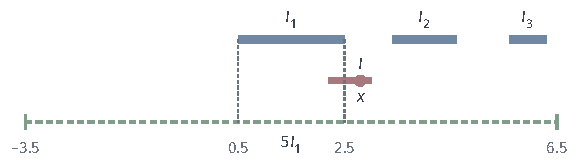
\includegraphics[width=97.991mm]{figures/04-spaces-measures-and-geometry/02-measure/tikz/integ-vitali-cover/figure.pdf}
  \caption{Vitali选择中的五倍放大。蓝色为已选的两两不交区间$I_1=[0.5,2.5]$、$I_2=[3.4,4.6]$、$I_3=[5.6,6.3]$；红色区间$I=[2.2,3.0]$含点$x$，与$I_1$相交且$\lvert I\rvert=0.8<2\lvert I_1\rvert$，因此落在与$I_1$同心、长为$10$的区间$5I_1=[-3.5,6.5]$（绿色虚线）中。}
  \label{fig:integ-vitali-cover}
\end{BookInlineFigure}

\paragraph{单调函数的导数}
为描述导数可能不存在的情况，对$x\in(a,b)$引入右侧差商$\bigl(F(x+h)-F(x)\bigr)/h$在$h\downarrow0$时的上极限$D^+F(x)$与下极限$D_+F(x)$，以及左侧差商$\bigl(F(x)-F(x-h)\bigr)/h$的上极限$D^-F(x)$与下极限$D_-F(x)$，统称\term{Dini导数}（Dini derivative）。$F$在$x$处可导当且仅当四者相等且有限。

下面的证明还要用到积分的平移不变性：对可积或非负可测的$\phi$与实数$h$，有
\[
 \int_{[a,b]}\phi(x+h)\,\mathrm dx=\int_{[a+h,b+h]}\phi(x)\,\mathrm dx .
\]
对指示函数这就是Lebesgue测度的平移不变性，由线性性推广到简单函数，再由递增逼近推广到非负可测函数和可积函数。

单调函数的增量总和被端点差控制，这个全局约束足以迫使差商在几乎每一点收敛。

\begin{theorem}[单调函数几乎处处可导]
\label{thm:integ-monotone-differentiable}
设$F:[a,b]\to\mathbb R$单调不减。则$F$在$[a,b]$上几乎处处有有限导数，$F'$（在导数不存在处取$0$）可积，并且
\begin{equation}
 \int_a^bF'(x)\,\mathrm dx\leq F(b)-F(a).
 \label{eq:integ-monotone-derivative-bound}
\end{equation}
\end{theorem}

\begin{proof}
先证四个Dini导数几乎处处相等。取有理数$0<u<v$，令
\[
 E=\{x\in(a,b):D_-F(x)<u<v<D^+F(x)\},\qquad s=\lambda^*(E).
\]
思路是用$E$上的两种差商夹出矛盾：左侧小区间上增量小于$u$倍长度，右侧小区间上增量大于$v$倍长度。

对$\varepsilon>0$取开集$O\supseteq E$，$\lambda(O)<s+\varepsilon$。每个$x\in E$都有任意小的$h>0$，使$[x-h,x]\subseteq O\cap(a,b)$且$F(x)-F(x-h)<uh$。这些区间构成$E$的Vitali覆盖，由引理~\ref{lem:integ-vitali}选出两两不交的$[x_k-h_k,x_k]$（$k\leq N$），未覆盖部分外测度小于$\varepsilon$，并且
\[
 \sum_k\bigl(F(x_k)-F(x_k-h_k)\bigr)<u\lambda(O)<u(s+\varepsilon).
\]

令$A$为$E$落在这些区间内部的部分，则$\lambda^*(A)>s-\varepsilon$。每个$y\in A$都有任意小的$k>0$，使$[y,y+k]$含于某个$(x_j-h_j,x_j)$且$F(y+k)-F(y)>vk$。再用引理选出两两不交的$J_1,\dots,J_M$，总长大于$s-2\varepsilon$，于是$F$在这些区间上的增量之和大于$v(s-2\varepsilon)$。

$F$单调不减，同一个$[x_k-h_k,x_k]$内不交子区间上的增量之和不超过它两端的增量。比较两次估计，得到
\[
 v(s-2\varepsilon)<u(s+\varepsilon).
\]
令$\varepsilon\to0$得$vs\leq us$。由$u<v$，只能$s=0$。

对所有有理数对取并，$D^+F\leq D_-F$几乎处处成立。把这一结论用于单调不减函数$\tilde F(x)=-F(-x)$，得到$D^-F\leq D_+F$几乎处处成立。于是几乎处处有
\[
 D^+F\leq D_-F\leq D^-F\leq D_+F\leq D^+F .
\]
四者相等，导数在$[0,+\infty]$中几乎处处存在。

再证积分估计，它同时说明导数几乎处处有限。对$x>b$令$F(x)=F(b)$，令$q_n(x)=n\bigl(F(x+1/n)-F(x)\bigr)$。单调函数的阈值集合是区间，所以$q_n$是非负可测函数，并在导数存在处$q_n\to F'$。由Fatou引理与平移不变性，
\[
\begin{aligned}
 \int_a^bF'\,\mathrm dx&\leq\liminf_n\int_a^bq_n\,\mathrm dx\\
 &=\liminf_n\Bigl(n\int_b^{b+1/n}F\,\mathrm dx-n\int_a^{a+1/n}F\,\mathrm dx\Bigr).
\end{aligned}
\]
在$[b,b+1/n]$上$F=F(b)$，在$[a,a+1/n]$上$F\geq F(a)$，所以右端不超过$F(b)-F(a)$。左侧有限，非负可积函数几乎处处有限。
\end{proof}

式~\eqref{eq:integ-monotone-derivative-bound}只是不等式。$[0,1]$上的阶跃函数$\mathbf 1_{[1/2,1]}$单调不减，除$x=1/2$外导数都是$0$，导数的积分为$0$，而端点增量为$1$；增量全部发生在一个点上，导数读不到它。所以单调性只给出导数的存在与总量的上界。

\paragraph{变上限积分的导数}
现在回到$G(x)=\int_a^xg$。证明思路是先得到$\int_a^c(G'-g)=0$对每个$c$成立，所以需要一个判零引理：区间上的积分全为零的函数几乎处处为零。

\begin{lemma}[区间积分全为零的函数]
\label{lem:integ-vanishing-intervals}
设$g$在$[a,b]$上可积且为实值。若对每个$x\in[a,b]$都有$\int_a^xg=0$，则$g=0$几乎处处成立。
\end{lemma}

\begin{proof}
Lebesgue可测函数与某个Borel函数几乎处处相等，改动零测集不影响结论，不妨设$g$是Borel函数。令$\mathcal D$为使$\int_Eg=0$的Borel集$E\subseteq[a,b]$全体。

区间$(c,d]\subseteq[a,b]$满足
\[
 \int_{(c,d]}g=\int_a^dg-\int_a^cg=0,
\]
这些区间与空集对有限交封闭，并生成$[a,b]$上的Borel集（单点零测，可以并入）。

$\mathcal D$是$\lambda$系统：$[a,b]\in\mathcal D$；补集由$\int_{E^c}g=\int g-\int_Eg$得到；两两不交的可数并由支配收敛（以$\lvert g\rvert$为控制）得到。由$\pi$--$\lambda$定理，$\mathcal D$包含全部Borel集。取$E=\{g>0\}$，得$\int g^+=0$，所以$g\leq0$几乎处处成立；同理$g\geq0$几乎处处成立。
\end{proof}

现在可以陈述本小节的主要结论。

\begin{theorem}[Lebesgue微分定理]
\label{thm:integ-lebesgue-differentiation}
设$g$在$[a,b]$上可积，$G$由式~\eqref{eq:integ-indefinite}给出。则$G$绝对连续，$G$几乎处处可导，并且$G'=g$几乎处处成立，即对几乎每个$x\in(a,b)$，
\begin{equation}
 \lim_{h\to0}\frac1h\int_x^{x+h}g(t)\,\mathrm dt=g(x).
 \label{eq:integ-lebesgue-differentiation}
\end{equation}
其中$h<0$时$\int_x^{x+h}$理解为$-\int_{x+h}^x$。
\end{theorem}

\begin{proof}
绝对连续性已经证明。复值情形对实部、虚部分别处理；实值情形由$g=g^+-g^-$与导数的线性性，只需对$g\geq0$证明。

先设$0\leq g\leq M$。此时$G$单调不减且是Lipschitz函数，由定理~\ref{thm:integ-monotone-differentiable}几乎处处可导。对$x>b$令$G(x)=G(b)$，差商$q_n(x)=n\bigl(G(x+1/n)-G(x)\bigr)$满足$0\leq q_n\leq M$，并在$G$可导处趋于$G'$。对$c\in(a,b]$，在$[a,c]$上以常数$M$为控制用支配收敛，再平移，得
\[
 \int_a^cG'\,\mathrm dx=\lim_{n\to\infty}\Bigl(n\int_c^{c+1/n}G\,\mathrm dx-n\int_a^{a+1/n}G\,\mathrm dx\Bigr).
\]
$G$连续，函数在缩小区间上的平均值趋于端点值，所以右端等于$G(c)-G(a)$。于是
\[
 \int_a^c(G'-g)\,\mathrm dx=0
\]
对所有$c$成立，由引理~\ref{lem:integ-vanishing-intervals}，$G'=g$几乎处处成立。

再看一般的$g\geq0$。令$g_n=\min\{g,n\}$，$G_n(x)=\int_a^xg_n$。由有界情形，$G_n'=g_n$几乎处处成立。函数$G-G_n=\int_a^x(g-g_n)$单调不减，其导数几乎处处非负，所以$G'\geq g_n$几乎处处成立；合并可数个例外集，得$G'\geq g$几乎处处成立。

另一方面，由式~\eqref{eq:integ-monotone-derivative-bound}，
\[
 \int_a^bG'\,\mathrm dx\leq G(b)-G(a)=\int_a^bg\,\mathrm dx .
\]
因此$G'-g\geq0$几乎处处成立且积分不超过$0$，由定理~\ref{thm:integ-monotonicity}，$G'=g$几乎处处成立。
\end{proof}

定理的名称来自式~\eqref{eq:integ-lebesgue-differentiation}：$g$在$x$附近的局部平均值，在几乎每一点恢复$g$的取值。卷一要求$g$连续，结论在每一点成立；这里$g$只是可积，结论在零测集外成立。

下面用一个能手算的例子看例外集。在$[0,2]$上取$g=\mathbf 1_{[0,1]}$，变上限积分是
\[
 G(x)=\min\{x,1\}.
\]
除$x=1$外$G$都可导，$x<1$时$G'=1=g$，$x>1$时$G'=0=g$；在$x=1$处$G$有折角，导数不存在。例外集是单点，与定理相符。

$[0,1]$上的$\mathbf 1_{\mathbb Q}$说明“几乎处处”不能改成“处处”：它的变上限积分恒为$0$，导数$0$与$\mathbf 1_{\mathbb Q}$在每个有理点都不同。

\subsection{由导数恢复函数}
\label{sec:integ-recovery}

\paragraph{有界变差与导数的存在}
现在处理第二个方向：给定绝对连续的$F$，要证明$F(x)=F(a)+\int_a^xF'$。第一步是确认$F'$几乎处处存在且可积。对$[a,b]$的分割$P:a=x_0<\dots<x_n=b$，令
\[
 V(F,P)=\sum_k\lvert F(x_k)-F(x_{k-1})\rvert .
\]
称$V_a^b(F)=\sup_PV(F,P)$为$F$在$[a,b]$上的变差，它是函数图像沿纵向走过的总路程；若它有限，称$F$为\term{有界变差函数}（function of bounded variation）。在分割中插入点只会使$V(F,P)$不减，所以变差对区间可加：$V_a^b(F)=V_a^c(F)+V_c^b(F)$。

\begin{lemma}[绝对连续函数有界变差]
\label{lem:integ-ac-bv}
若$F$在$[a,b]$上绝对连续，则$F$是有界变差函数，并且是两个单调不减函数之差。
\end{lemma}

\begin{proof}
对$\varepsilon=1$取定义中的$\delta$，把$[a,b]$等分成$K$段，每段长度小于$\delta$。在一段$[c,d]$内任取分割，其小区间两两不交、总长小于$\delta$，增量之和小于$1$，故$V_c^d(F)\leq1$。由区间可加性，$V_a^b(F)\leq K$。

令$V(x)=V_a^x(F)$。对$x<y$，$V(y)-V(x)=V_x^y(F)\geq\lvert F(y)-F(x)\rvert$，所以$V$与$V-F$都单调不减，而$F=V-(V-F)$。
\end{proof}

由定理~\ref{thm:integ-monotone-differentiable}，两个单调函数都几乎处处可导且导数可积，所以绝对连续函数$F$几乎处处可导，$F'$可积。

\paragraph{零导数引理}
令$H(x)=F(x)-F(a)-\int_a^xF'$。由上一小节，$H$绝对连续且$H'=F'-F'=0$几乎处处成立。恢复公式就归结为：导数几乎处处为零的绝对连续函数必为常数。阶跃函数说明没有绝对连续性时这不成立；绝对连续性的作用，是控制导数为零的点之外那些总长很小的间隙上的增量。

\begin{lemma}[零导数引理]
\label{lem:integ-zero-derivative}
若$H$在$[a,b]$上绝对连续，且$H'=0$几乎处处成立，则$H$是常数。
\end{lemma}

\begin{proof}
任取$c\in(a,b]$，证明$H(c)=H(a)$。给定$\varepsilon>0$，取绝对连续定义中的$\delta$。令$E=\{x\in(a,c):H'(x)=0\}$，则$\lambda(E)=c-a$。

对每个$x\in E$，有任意小的$h>0$使$[x,x+h]\subseteq(a,c)$且$\lvert H(x+h)-H(x)\rvert<\varepsilon h$。这些区间构成$E$的Vitali覆盖，由引理~\ref{lem:integ-vitali}选出两两不交的$[x_k,y_k]$（$k=1,\dots,N$，按$x_1<y_1<x_2<\dots<y_N$排列），使$\lambda\bigl(E\setminus\bigcup_k[x_k,y_k]\bigr)<\delta$。

记$y_0=a$、$x_{N+1}=c$。剩下的间隙$(y_k,x_{k+1})$两两不交，总长小于$\delta$。把端点增量沿选中区间和间隙拆开：
\[
 \lvert H(c)-H(a)\rvert\leq\sum_{k=1}^N\lvert H(y_k)-H(x_k)\rvert+\sum_{k=0}^N\lvert H(x_{k+1})-H(y_k)\rvert .
\]
第一个和由导数为零控制，不超过$\varepsilon\sum_k(y_k-x_k)\leq\varepsilon(c-a)$；第二个和由绝对连续性控制，小于$\varepsilon$。于是
\[
 \lvert H(c)-H(a)\rvert<\varepsilon(c-a)+\varepsilon .
\]
$\varepsilon$任意，所以$H(c)=H(a)$。
\end{proof}

\paragraph{恢复公式}
零导数引理补上了最后一步，两个方向合起来给出一个双向刻画。

\begin{theorem}[Lebesgue微积分基本定理]
\label{thm:integ-ftc}
设$F:[a,b]\to\mathbb R$。以下两条等价：
\begin{enumerate}
 \item $F$在$[a,b]$上绝对连续；
 \item 存在$[a,b]$上的可积函数$g$，使$F(x)=F(a)+\int_a^xg(t)\,\mathrm dt$对所有$x\in[a,b]$成立。
\end{enumerate}
此时$F$几乎处处可导，$F'=g$几乎处处成立，并且对任意$c,x\in[a,b]$，
\begin{equation}
 F(x)=F(c)+\int_c^xF'(t)\,\mathrm dt,
 \label{eq:integ-ftc}
\end{equation}
其中$x<c$时$\int_c^x$理解为$-\int_x^c$。
\end{theorem}

\begin{proof}
(2)推出(1)及$F'=g$几乎处处成立，就是定理~\ref{thm:integ-lebesgue-differentiation}。

(1)推出(2)。由引理~\ref{lem:integ-ac-bv}，$F'$几乎处处存在且可积。令$H(x)=F(x)-F(a)-\int_a^xF'$，它绝对连续且$H'=0$几乎处处成立。由引理~\ref{lem:integ-zero-derivative}，$H\equiv H(a)=0$，取$g=F'$即得(2)。

式~\eqref{eq:integ-ftc}由$x$与$c$两处的(2)相减得到。
\end{proof}

这一形式的\term{微积分基本定理}（fundamental theorem of calculus）说：绝对连续函数恰好是可积函数的变上限积分加上常数，这个可积函数在几乎处处的意义下唯一确定为$F'$。

式~\eqref{eq:integ-ftc}说明怎样恢复整个函数：只需知道一点的函数值$F(c)$和一个可积的导数代表。导数在零测集上的取值无关紧要，函数值却要在一点给定，否则只能恢复到相差一个常数。

例如$F(x)=\lvert x\rvert$在$[-1,1]$上是Lipschitz函数，因而绝对连续。除$x=0$外$F'(x)=\operatorname{sgn}x$。从$c=-1$出发恢复，
\[
 F(0)=F(-1)+\int_{-1}^0(-1)\,\mathrm dt=1-1=0,
\]
再继续恢复到右端点，
\[
 F(1)=F(0)+\int_0^11\,\mathrm dt=1 .
\]
两个值都与$\lvert x\rvert$一致；$F'$在$x=0$处没有定义，并不影响恢复。

\paragraph{Cantor函数}
仅有连续性和几乎处处可导，还不能保证恢复公式。下面用Cantor集构造一个反例。记第~\ref{chap:measure}章Cantor集构造中第$n$步的$2^n$个保留闭区间之并为$C_n$。令$c_n:[0,1]\to[0,1]$是这样的连续分段线性函数：$c_n(0)=0$，在$C_n$的每个保留区间上线性增加$2^{-n}$，在已删去的开区间上取常值，于是$c_n(1)=1$。

从$c_n$到$c_{n+1}$，在每个保留区间上，原来线性增加的$2^{-n}$被分成左、右三分之一上各增加$2^{-n-1}$，中间三分之一上不变；两端的值不变。在同一个保留区间上，$c_n$与$c_{n+1}$都是单调函数，从相同的起点走到相同的终点，总上升量是$2^{-n}$，所以二者之差不超过$2^{-n}$。在已删去的区间上二者相等。于是
\[
 \sup_{[0,1]}\lvert c_{n+1}-c_n\rvert\leq2^{-n}.
\]
所以$c_n$一致收敛到一个连续函数$c$，称为\term{Cantor函数}（Cantor function）。它单调不减，$c(0)=0$，$c(1)=1$，并且在每个删去的开区间上取常值，因为从删去这一区间的那一步起，所有$c_n$在其上都取同一个常值。图~\ref{fig:integ-cantor-function}画出了前几步的逼近。

\begin{BookInlineFigure}
  \centering
  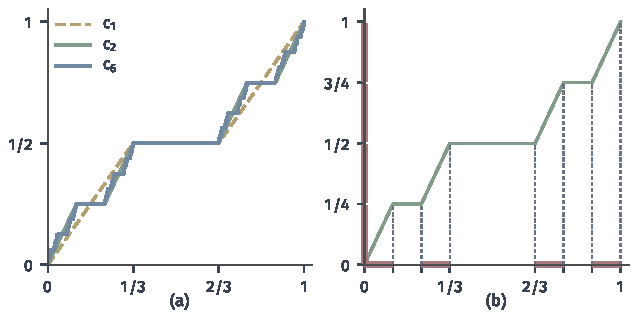
\includegraphics[width=108mm]{figures/04-spaces-measures-and-geometry/02-measure/matplotlib/integ-cantor-function/figure.pdf}
  \caption{Cantor函数及其分段线性逼近。(a)$c_1$（黄色虚线）、$c_2$（绿）与$c_6$（蓝），$c_n$在第$n$步的$2^n$个保留区间上线性增加$2^{-n}$，在已删去的区间上保持常值。(b)第二步的四个保留区间$[0,\frac19]$、$[\frac29,\frac13]$、$[\frac23,\frac79]$、$[\frac89,1]$（横轴红色）总长$\frac49$，对应的增量（纵轴红色）各为$\frac14$，合起来覆盖整个$[0,1]$。}
  \label{fig:integ-cantor-function}
\end{BookInlineFigure}

$[0,1]\setminus C$是删去的开区间之并，$c$在其中每一点导数为$0$；$\lambda(C)=0$，所以$c'=0$几乎处处成立，而
\[
 \int_0^1c'(x)\,\mathrm dx=0\neq1=c(1)-c(0).
\]
恢复公式失败，由定理~\ref{thm:integ-ftc}，$c$不绝对连续。这也可以直接从定义看出：第$n$步的$2^n$个保留区间（取其内部）两两不交，总长$(2/3)^n\to0$，$c$在它们上的增量之和始终是$1$。

Cantor函数把几种容易混淆的性质分开了。它连续，所以连续不能保证恢复公式；它单调，因而有界变差并且几乎处处可导，所以这两条也不够；它缺的正是绝对连续性。在$[a,b]$上有
\begin{equation}
 \text{Lipschitz}\Rightarrow\text{绝对连续}\Rightarrow\text{连续且有界变差}\Rightarrow\text{几乎处处可导},
 \label{eq:integ-regularity-chain}
\end{equation}
三个箭头都不能反过来，反例依次是$\sqrt x$、Cantor函数与阶跃函数$\mathbf 1_{[1/2,1]}$。

Cantor函数作为Stieltjes测度的累积函数，给出一个没有点质量、却集中在零测集$C$上的概率测度；第~\ref{chap:measure-densities}章把实轴上的测度分解为点质量、绝对连续与这类奇异连续三部分时，它是奇异连续部分的标准例子。

\section{含参积分}
\label{sec:integ-parametric}

很多量由一个依赖参数的积分给出，例如$F(t)=\int_0^\infty e^{-tx}\,\mathrm dx$，或下一章的局部平均$\int\rho_\varepsilon(x-y)f(y)\,\mathrm dy$。我们关心$F$作为参数的函数是否连续、是否可导，导数能否移到积分号内计算。这些问题都可以化为函数列的积分极限：参数$t_n\to t$时，被积函数$f(\cdot,t_n)$构成一列函数，差商构成另一列函数。所以支配收敛定理是本节的主要工具，关键是找出合适的共同上界。先处理固定的积分区域，再讨论积分区域随参数移动时的额外变化。

\subsection{积分对参数的连续性}
\label{sec:integ-parameter-continuity}

\paragraph{连续性定理}
设$(X,\mathcal A,\mu)$是测度空间，参数$t$取值于度量空间$T$，$f:X\times T\to\mathbb C$，并且每个$f(\cdot,t)$可测。令$F(t)=\int_Xf(x,t)\,\mathrm d\mu(x)$。被积函数关于参数的逐点连续性不足以推出$F$连续，还需要一个与参数无关的可积上界，防止质量在参数变化时逃逸。

\begin{theorem}[含参积分的连续性]
\label{thm:integ-parameter-continuity}
设$t_0\in T$，$U$是$t_0$的邻域。若存在零测集$N$与可积函数$g\geq0$，使对每个$x\notin N$：
\begin{enumerate}
 \item $t\mapsto f(x,t)$在$t_0$处连续；
 \item 对一切$t\in U$，$\lvert f(x,t)\rvert\leq g(x)$，
\end{enumerate}
则$F$在$U$上有定义，并在$t_0$处连续。
\end{theorem}

\begin{proof}
由第2条，每个$f(\cdot,t)$（$t\in U$）可积，$F$在$U$上有定义。度量空间中的连续性可以用序列检验：任取$t_n\to t_0$，不妨设$t_n\in U$。函数列$f(\cdot,t_n)$在$N$外收敛到$f(\cdot,t_0)$，并由同一个$g$控制。由支配收敛定理，$F(t_n)\to F(t_0)$。
\end{proof}

定理要求的控制是对参数邻域内\emph{所有}$t$同时成立的：控制的是参数变化后的函数值，而不只是$t_0$处的函数值。零测集$N$也必须与$t$无关，因为参数可以取不可数多个值，而不可数个零测例外的并不一定零测。

例如$F(t)=\int_0^\infty e^{-x}\cos(tx)\,\mathrm dx$。对每个$x$，$t\mapsto e^{-x}\cos(tx)$连续，并且$\lvert e^{-x}\cos(tx)\rvert\leq e^{-x}$对一切$t\in\mathbb R$成立，$e^{-x}$在$[0,\infty)$上可积，所以$F$在$\mathbb R$上处处连续。

\paragraph{控制失效的情形}
在$[0,\infty)$上取$f(x,t)=te^{-tx}$，$t\geq0$。对每个固定的$x>0$，$t\mapsto te^{-tx}$连续，在$t=0$处取$0$。但$t>0$时$F(t)=\int_0^\infty te^{-tx}\,\mathrm dx=1$，而$F(0)=0$，$F$在$0$处不连续。

图~\ref{fig:integ-parameter-continuity}显示了原因：$t$越小，曲线越低、越向右摊开，面积始终为$1$；质量没有消失，而是逃向无穷远处。任何控制函数都不小于包络$\sup_{t>0}te^{-tx}=1/(ex)$（在$t=1/x$处取到），它在无穷远处不可积，所以$t=0$附近不存在可积的共同上界。与尖峰例子相比，这里质量不是挤进窄区间，而是摊到无界区域上，支配条件同样排除了这种情况。

\begin{figure}[!htbp]
\centering
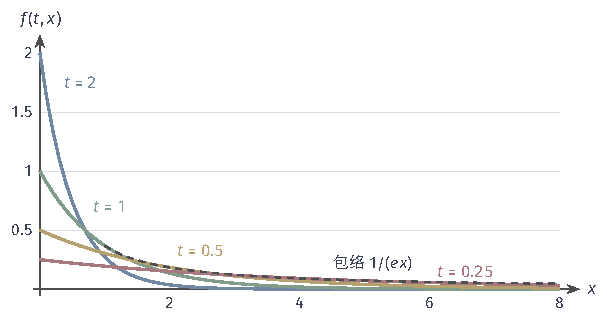
\includegraphics[width=102.807mm]{figures/02-abstract-mathematics/01-metric-and-measure/tikz/c3-parameter-continuity/figure.pdf}
\caption{含参积分中质量的逃逸。四条实线是$f(t,x)=te^{-tx}$在$t=2,1,0.5,0.25$时的图像，每条曲线下的面积都是$1$；$t$越小，质量越向右摊开。虚线是包络$\sup_tte^{-tx}=1/(ex)$（在$t=1/x$处取到，画在$x\geq1$部分），它在无穷远处不可积，所以$t=0$附近没有可积控制。}
\label{fig:integ-parameter-continuity}
\end{figure}

\subsection{积分号下求导}
\label{sec:integ-differentiation-under-integral}

\paragraph{求导定理}
现在设参数取值于开区间$T\subseteq\mathbb R$。$F$在$t$处的差商是$\int\bigl(f(x,t+h)-f(x,t)\bigr)/h\,\mathrm d\mu$，被积函数在$h\to0$时趋于$\partial_tf(x,t)$。要把极限移进积分号，同样需要给差商一个共同的可积上界；由中值定理，差商的大小由导数在参数区间上的大小控制。

\begin{theorem}[积分号下求导]
\label{thm:integ-differentiation-under-integral}
设$T\subseteq\mathbb R$是开区间，$f:X\times T\to\mathbb R$满足：
\begin{enumerate}
 \item 存在$t_0\in T$，使$f(\cdot,t_0)$可积；
 \item 存在零测集$N$，使对每个$x\notin N$，$t\mapsto f(x,t)$在$T$上可微；
 \item 存在可积函数$g\geq0$，使对每个$x\notin N$与每个$t\in T$，$\lvert\partial_tf(x,t)\rvert\leq g(x)$。
\end{enumerate}
则对每个$t\in T$，$f(\cdot,t)$可积，$F(t)=\int_Xf(x,t)\,\mathrm d\mu(x)$在$T$上可微，并且
\[
 F'(t)=\int_X\partial_tf(x,t)\,\mathrm d\mu(x).
\]
复值函数对实部与虚部分别应用即可。
\end{theorem}

\begin{proof}
对$x\notin N$，由中值定理，$\lvert f(x,t)-f(x,s)\rvert\leq g(x)\lvert t-s\rvert$对$s,t\in T$成立。取$s=t_0$，得$\lvert f(x,t)\rvert\leq\lvert f(x,t_0)\rvert+\lvert t-t_0\rvert g(x)$，右边可积，所以每个$f(\cdot,t)$可积。

固定$t\in T$，任取$h_n\to0$且$t+h_n\in T$，$h_n\neq0$。差商$q_n(x)=\bigl(f(x,t+h_n)-f(x,t)\bigr)/h_n$是可测函数，在$N$外收敛到$\partial_tf(x,t)$，所以$\partial_tf(\cdot,t)$在$N$外是可测函数列的极限，可测。由中值定理，$\lvert q_n(x)\rvert\leq g(x)$。由支配收敛定理与线性性，
\[
 \frac{F(t+h_n)-F(t)}{h_n}=\int_Xq_n\,\mathrm d\mu\to\int_X\partial_tf(x,t)\,\mathrm d\mu .
\]
对一切$h_n\to0$都成立，所以$F$在$t$处可微且导数如定理所述。
\end{proof}

导数的控制条件只需在一个参数区间内成立。若条件只在每个$t$附近的某个子区间上成立，把定理用于这些子区间，同样得到$F$在整个$T$上可微。

\begin{example}[逐阶求导]
\label{ex:integ-gamma-derivatives}
对$t>0$，$F(t)=\int_0^\infty e^{-tx}\,\mathrm dx=1/t$。固定$t_0>0$，在$T=(t_0,\infty)$上，$\lvert\partial_te^{-tx}\rvert=xe^{-tx}\leq xe^{-t_0x}$，右边在$[0,\infty)$上可积。由定理，$-\int_0^\infty xe^{-tx}\,\mathrm dx=F'(t)=-1/t^2$。同样的控制$x^ne^{-t_0x}$允许继续求导，归纳得$\int_0^\infty x^ne^{-tx}\,\mathrm dx=n!/t^{n+1}$；取$t=1$即$\int_0^\infty x^ne^{-x}\,\mathrm dx=n!$。由于$t_0>0$任意，结论对一切$t>0$成立；而在$t=0$附近控制失效，$F$本身也在那里趋于无穷。
\end{example}

\paragraph{偏导数逐点存在不等于可以交换}
定理的第3条不能省去。在$[0,\infty)$上取$f(x,t)=t^3e^{-t^2x}$，$t\in\mathbb R$。对$t\neq0$，$F(t)=t^3\cdot t^{-2}=t$；又$F(0)=0$，所以$F(t)=t$，$F'(0)=1$。另一方面，对每个$x\geq0$，
\[
 \partial_tf(x,0)=\lim_{t\to0}\frac{t^3e^{-t^2x}}t=0,
\]
于是$\int_0^\infty\partial_tf(x,0)\,\mathrm dx=0\neq1$。偏导数在每一点都存在，交换却失败了。原因是$\partial_tf(x,t)=(3t^2-2t^4x)e^{-t^2x}$在$t^2=1/x$处等于$1/(ex)$，所以在$0$的任何参数邻域内，它的上包络不小于一个在无穷远处不可积的函数；控制条件必须覆盖参数邻域，只在$t=0$处检查导数是不够的。

\subsection{变动区域上的积分}
\label{sec:integ-moving-domain}

\paragraph{变限的一元积分}
当积分区域也随参数移动时，$F(t)$的变化来自两部分：区域内部的被积函数在变，边界又新添或移除了一部分区域。先看一元的变限积分$F(t)=\int_{a(t)}^{b(t)}f(x,t)\,\mathrm dx$。

\begin{theorem}[变限积分的求导]
\label{thm:integ-variable-limits}
设$J=[\alpha,\beta]$，$T\subseteq\mathbb R$是开区间，$a,b:T\to J$可微。设$f:J\times T\to\mathbb R$连续，$\partial_tf$在$J\times T$上处处存在，并存在可积函数$g\geq0$使$\lvert\partial_tf(x,t)\rvert\leq g(x)$对一切$x\in J$、$t\in T$成立。则$F(t)=\int_{a(t)}^{b(t)}f(x,t)\,\mathrm dx$在$T$上可微，且
\[
 F'(t)=\int_{a(t)}^{b(t)}\partial_tf(x,t)\,\mathrm dx+f\bigl(b(t),t\bigr)b'(t)-f\bigl(a(t),t\bigr)a'(t).
\]
\end{theorem}

\begin{proof}
固定$t$，取$h\neq0$且$t+h\in T$，记$a=a(t)$、$a_h=a(t+h)$，$b,b_h$同理。把增量拆成三部分：
\begin{equation*}
\begin{aligned}
 F(t+h)-F(t)={}&\int_a^b\bigl(f(x,t+h)-f(x,t)\bigr)\mathrm dx\\
 &+\int_b^{b_h}f(x,t+h)\,\mathrm dx-\int_a^{a_h}f(x,t+h)\,\mathrm dx .
\end{aligned}
\end{equation*}
第一项除以$h$后，由定理~\ref{thm:integ-differentiation-under-integral}的论证（差商由$g$控制，支配收敛）趋于$\int_a^b\partial_tf(x,t)\,\mathrm dx$。

第二项来自上端点的移动。$f$在$(b,t)$处连续，对$\varepsilon>0$，当$h$足够小时，$b_h$与$b$之间的每个$x$都满足$\lvert f(x,t+h)-f(b,t)\rvert<\varepsilon$。于是
\[
 \Bigl\lvert\frac1h\int_b^{b_h}f(x,t+h)\,\mathrm dx-\frac{b_h-b}hf(b,t)\Bigr\rvert\leq\varepsilon\Bigl\lvert\frac{b_h-b}h\Bigr\rvert,
\]
而$(b_h-b)/h\to b'(t)$，所以第二项除以$h$趋于$f(b,t)b'(t)$。第三项同理趋于$f(a,t)a'(t)$。
\end{proof}

两个边界项符号相反：上端向右移动增加积分区域，下端向右移动减少积分区域。例如$F(t)=\int_0^txt\,\mathrm dx=t^3/2$，直接求导得$3t^2/2$；按定理计算，内部变化贡献$\int_0^tx\,\mathrm dx=t^2/2$，上端移动贡献$f(t,t)\cdot1=t^2$，合计$3t^2/2$，两者一致。与卷二在连续可微条件下的同一公式相比，这里只要求被积函数连续、参数导数有可积控制，内部项的交换完全由支配收敛负责；连续性只在边界点上用于读出新添部分的高度。

\paragraph{有参数的多元区域}
在$\mathbb R^d$中，区域的移动不能只用两个端点描述，需要把区域参数化。设$\Omega_0\subseteq\mathbb R^d$是开集，对每个$t\in T$，$\Phi_t:\Omega_0\to\Omega_t$是连续可微的双射，逆映射也连续可微，记$J_t(y)=\lvert\det D\Phi_t(y)\rvert$。由卷二的积分换元公式（可参考\BookChapterRef{chap:region-integrals}{卷二第21章“区域积分”}），
\[
 F(t)=\int_{\Omega_t}f(x,t)\,\mathrm dx=\int_{\Omega_0}f\bigl(\Phi_t(y),t\bigr)J_t(y)\,\mathrm dy,
\]
右端是固定区域上的积分。

于是变动区域的问题化为固定区域上的含参积分：只要对几乎每个$y$，映射$t\mapsto f(\Phi_t(y),t)J_t(y)$可微，并且这个参数导数在$T$上有与$t$无关的可积上界，就可以用定理~\ref{thm:integ-differentiation-under-integral}在积分号下求导。这里有两类条件：边界的移动由参数化$\Phi_t$的光滑性描述，被积函数的变化由支配条件控制，二者都要在使用前核对。一元情形取$\Phi_t(y)=a(t)+y(b(t)-a(t))$，$\Omega_0=(0,1)$，得到的正是上面的公式。

在$\Phi$足够光滑时，把导数写回$\Omega_t$上，并用散度定理把与区域移动有关的部分改写成边界上的通量，可以得到边界项的多元形式：它沿整个边界累计被积函数乘以边界的法向移动速度。这一改写需要边界的光滑性与散度定理，这里不展开推导。

\section{本章小结}
\label{sec:integ-summary}

本章开头问：怎样按位置给出不同的贡献再累计，累计能否与极限、依次求积和求导交换。积分按值域分层：非负简单函数的积分是“高度乘以测度”之和，与写法无关；一般非负可测函数的积分是下方简单函数积分的上确界，允许取$+\infty$，并且任何一列递增的简单逼近都能算出它。实值函数把正部与负部分开累计，只要至少一部分有限积分就存在，两部分都有限才称可积；复值函数以模的积分有限为可积条件，按实部与虚部积分。积分看不见零测集，只依赖函数的几乎处处等价类。

基本性质各有条件。非负函数的线性组合要求系数非负，并按$0\cdot(+\infty)=0$处理无穷；可积函数允许任意实系数或复系数，但只知道积分存在不足以相加。单调性可以放宽到几乎处处，复值积分不比较大小，绝对值估计则通过旋转把复积分化为实部与模的比较，并给出$\lvert\int f-\int g\rvert\leq\int\lvert f-g\rvert$。有限个不交区域的积分可加，增删零测集不改变积分，可数个区域的情形要用单调收敛定理。

与经典积分相比，有界闭区间上的有界函数黎曼可积当且仅当不连续点集零测，此时两种积分相等；$\mathbf 1_{\mathbb Q}$只有新积分。反常积分在绝对收敛时与新积分一致，条件收敛的$\sin x/x$却不是Lebesgue可积的，因为测度积分不依赖任何次序。

积分与极限的交换由尖峰例子引出：逐点收敛不足以保证积分收敛，质量可以挤进越来越窄的区间，或者摊到无界区域上。单调收敛定理处理递增的非负函数列，并给出非负级数逐项积分；Fatou引理对非负函数列给出单向估计；支配收敛定理在存在共同可积上界时交换极限与积分，并保证$\int\lvert f_n-f\rvert\to0$。

累次积分与含参积分分别给出换序与参数运算的条件。$\sigma$有限测度的乘积测度由矩形上的乘积赋值唯一确定；Tonelli定理对非负可测函数无条件换序，Fubini定理在先核对$\int\lvert f\rvert<+\infty$后对一般函数换序，截面只需几乎处处可积，例外处的内层积分取零；完备化下截面的可测性也只对几乎每个参数成立。含参积分的连续性与积分号下求导都依赖参数邻域上与参数无关的可积控制；积分区域移动时，还要加上边界移动带来的项。

微积分基本定理在绝对连续条件下联系积分与导数。可积函数的变上限积分绝对连续，几乎处处可导，导数几乎处处等于被积函数；反过来，绝对连续函数几乎处处可导、导数可积，并能由一点的函数值和导数的积分恢复。Cantor函数连续、单调、几乎处处导数为零却从$0$增到$1$，标出了恢复公式的边界。第~\ref{chap:smoothing-weak-derivatives}章在这些基础上研究卷积光滑化与弱导数，那里要用到本章的换序、积分号下求导与一维的积分恢复；换测度与沿映射换元分别在第~\ref{chap:measure-densities}章与第~\ref{chap:pushforward-measures}章展开。

